\documentclass[12pt]{article}
\usepackage{amsmath,amssymb}
\usepackage{tikz}
\usetikzlibrary{arrows.meta, positioning, calc, decorations.markings}
\usepackage{comment} 
\usepackage[margin=1in]{geometry}

\title{Notes on the Hodge-deRham Complex}

\author{John A. Janik}

\begin{document}
	
\maketitle

\begin{comment}
\begin{center}
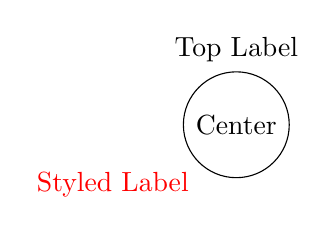
\begin{tikzpicture}
	\node[draw, circle,
	label=above:Top Label,
	label={[text=red]below left:Styled Label}] (n1) at (0,0) {Center};
\end{tikzpicture}
\end{center}

\draw[red, thick] (node1) -- (node2);
\draw[blue, very thick] (nodeA) -- (nodeB);

\draw[line width=1.5pt, green!60!black] (A) -- (B);
\draw[dashed, blue, ultra thick] (A) -- (B);

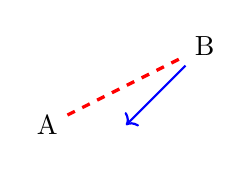
\begin{tikzpicture}[
	myline/.style={draw=red, very thick, dashed},
	arrowline/.style={->, blue, thick}
	]
	\node (A) at (0,0) {A};
	\node (B) at (2,1) {B};
	
	\draw[myline] (A) -- (B);
	\draw[arrowline] (B) -- (1,0);
\end{tikzpicture}



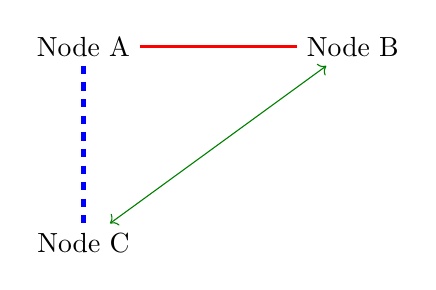
\begin{tikzpicture}[node distance=2cm]
	% Define nodes
	\node (A) {Node A};
	\node (B) [right=of A] {Node B};
	\node (C) [below=of A] {Node C};
		
	% Line 1: Thick Red
	\draw[red, very thick] (A) -- (B);
		
	% Line 2: Blue dashed, custom thickness
	\draw[blue, dashed, line width=2pt] (A) -- (C);
		
	% Line 3: Thin, dark green with arrows
	\draw[<->, green!50!black, thin] (B) -- (C);
\end{tikzpicture}
\end{comment}




\begin{center}
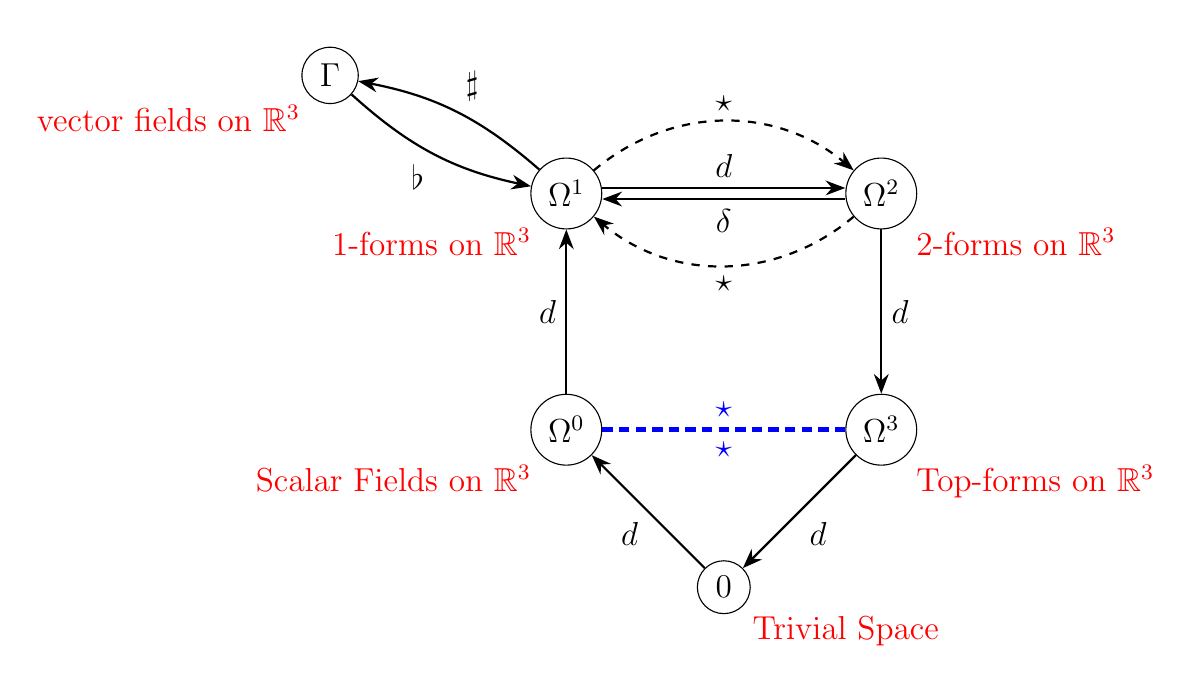
\begin{tikzpicture}[
    node distance=2.5cm and 3cm,
    every node/.style={font=\large},
    % Standard arrow
    arrow/.style={-{Stealth[length=2.5mm]}, thick},
    %reddash/.style={draw=red, very thick, dashed},
    myarrow/.style={->, blue, thick}
    % Musical isomorphism arrows (decorative)
    musical/.style={-{Stealth[length=2mm, width=2mm]}, thick, 
                    looseness=0.8},
    % Double parallel arrows style
    parallel shift/.style={transform canvas={yshift=#1}}
]

% === NODES ===

% Zero at bottom center
	\node [draw, circle,
	label=above:,
	label={[text=red]below right:Trivial Space}](zero) at (0,-3.5) {$0$};

% Middle row: Ω⁰ and Ω³
	\node [draw, circle,
	label=above:,
	label={[text=red]below left:Scalar Fields on $\mathbb{R}^{3}$}](omega0) at (-2, -1.5) {$\Omega^0$};
	\node [draw, circle,
		label=above:,
		label={[text=red]below right:Top-forms on $\mathbb{R}^{3}$}] (omega3) at (2, -1.5) {$\Omega^3$};

% Top row: $\omega^{1}$ and $\omega^{2}$
	\node [draw, circle,
	label=above:,
	label={[text=red]below left:1-forms on $\mathbb{R}^{3}$}] (omega1) at (-2, 1.5) {$\Omega^1$};
	\node [draw, circle,
	label=above:,
	label={[text=red]below right:2-forms on $\mathbb{R}^{3}$}](omega2) at (2, 1.5) {$\Omega^2$};

% Gamma in upper left corner
	\node [draw, circle,
	label=above:,
	label={[text=red]below left:vector fields on $\mathbb{R}^{3}$}] (Gamma) at (-5, 3) {$\Gamma$};

% === DE RHAM COMPLEX ARROWS (d) ===

% 0 → Ω⁰
\draw[arrow] (zero) -- node[midway, below left] {$d$} (omega0);


% Ω⁰ → $\omega^{1}$
\draw[arrow] (omega0) -- node[midway, left] {$d$} (omega1);

% $\omega^{1}$ → $\omega^{2}$ (upper parallel arrow)
\draw[arrow, parallel shift=2pt] (omega1) -- node[midway, above] {$d$} (omega2);

% $\omega^{2}$ → $\omega^{1}$ (lower parallel arrow, reversed for codifferential δ)
\draw[arrow, parallel shift=-2pt] (omega2) -- node[midway, below] {$\delta$} (omega1);

% $\omega^{2}$ → Ω³
\draw[arrow] (omega2) -- node[midway, right] {$d$} (omega3);

% Ω³ → 0
\draw[arrow] (omega3) -- node[midway, below right] {$d$} (zero);

% === HODGE STAR ARROWS (★) ===
%TTD: Add label "Hodge Isomorphisms" above blue line for Hodge Star
arrowline/.style={->, blue, thick}
% Ω⁰ $\leftrightarrow$ Ω³ (horizontal, parallel)
	%\draw[blue, dashed, line width=2pt] (omega0) -- (omega3);
	\draw[blue, dashed, line width=2pt]  (omega0) -- node[midway, above] {$\star$} (omega3);
	\draw[blue, dashed, line width=2pt] (omega3) -- node[midway, below] {$\star$} (omega0);

% $\omega^{1}$ $\leftrightarrow$ $\omega^{2}$ - already have d/δ, so we can add curved ★ or skip
% If you want ★ between $\omega^{1}$ and $\omega^{2}$, we need to distinguish from d/δ
% Option: use dashed or different style
\draw[arrow, dashed, bend left=40] (omega1) to node[midway, above] {$\star$} (omega2);
\draw[arrow, dashed, bend left=40] (omega2) to node[midway, below] {$\star$} (omega1);

% === MUSICAL ISOMORPHISMS (♭ and ♯) ===

% $\Gamma$ → $\omega^{1}$ (flat: ♭)
\draw[-{Stealth[length=2.5mm]}, thick, bend right=15] 
    (Gamma) to node[midway, below left] {$\flat$} (omega1);

% $\omega^{1}$ → $\Gamma$ (sharp: ♯)  
\draw[-{Stealth[length=2.5mm]}, thick, bend right=15] 
    (omega1) to node[midway, above right] {$\sharp$} (Gamma);

\end{tikzpicture}
\end{center}

\vspace{1cm}

%Above version but without the labes: Under contruction
\begin{center}
	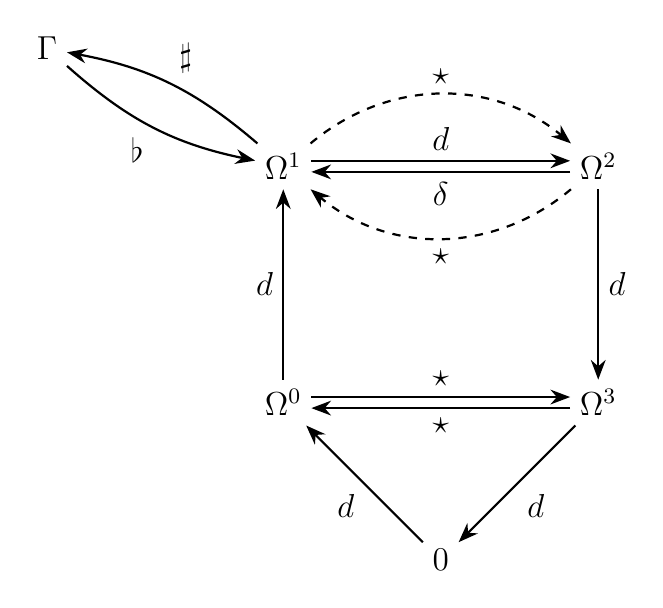
\begin{tikzpicture}[
		node distance=2.5cm and 3cm,
		every node/.style={font=\large},
		% Standard arrow
		arrow/.style={-{Stealth[length=2.5mm]}, thick},
		% Musical isomorphism arrows (decorative)
		musical/.style={-{Stealth[length=2mm, width=2mm]}, thick, 
			looseness=0.8},
		% Double parallel arrows style
		parallel shift/.style={transform canvas={yshift=#1}}
		]
		
		% === NODES ===
		
		% Zero at bottom center
		\node (zero) at (0,-3.5) {$0$};
		%\node[options, label={[label options]right=of zero}] (zero) at (0,-3.5) {$0$};
		
		
		% Middle row: Ω⁰ and Ω³
		\node (omega0) at (-2, -1.5) {$\Omega^0$};
		\node (omega3) at (2, -1.5) {$\Omega^3$};
		
		% Top row: $\omega^{1}$ and $\omega^{2}$
		\node (omega1) at (-2, 1.5) {$\Omega^1$};
		\node (omega2) at (2, 1.5) {$\Omega^2$};
		
		% Gamma in upper left corner
		\node (Gamma) at (-5, 3) {$\Gamma$};
		
		% === DE RHAM COMPLEX ARROWS (d) ===
		
		% 0 → Ω⁰
		\draw[arrow] (zero) -- node[midway, below left] {$d$} (omega0);
		
		% Ω⁰ → $\omega^{1}$
		\draw[arrow] (omega0) -- node[midway, left] {$d$} (omega1);
		
		% $\omega^{1}$ → $\omega^{2}$ (upper parallel arrow)
		\draw[arrow, parallel shift=2pt] (omega1) -- node[midway, above] {$d$} (omega2);
		
		% $\omega^{2}$ → $\omega^{1}$ (lower parallel arrow, reversed for codifferential δ)
		\draw[arrow, parallel shift=-2pt] (omega2) -- node[midway, below] {$\delta$} (omega1);
		
		% $\omega^{2}$ → Ω³
		\draw[arrow] (omega2) -- node[midway, right] {$d$} (omega3);
		
		% Ω³ → 0
		\draw[arrow] (omega3) -- node[midway, below right] {$d$} (zero);
		
		% === HODGE STAR ARROWS (★) ===
		
		% Ω⁰ $\leftrightarrow$ Ω³ (horizontal, parallel)
		\draw[arrow, parallel shift=2pt] (omega0) -- node[midway, above] {$\star$} (omega3);
		\draw[arrow, parallel shift=-2pt] (omega3) -- node[midway, below] {$\star$} (omega0);
		
		% $\omega^{1}$ $\leftrightarrow$ $\omega^{2}$ - already have d/δ, so we can add curved ★ or skip
		% If you want ★ between $\omega^{1}$ and $\omega^{2}$, we need to distinguish from d/δ
		% Option: use dashed or different style
		\draw[arrow, dashed, bend left=40] (omega1) to node[midway, above] {$\star$} (omega2);
		\draw[arrow, dashed, bend left=40] (omega2) to node[midway, below] {$\star$} (omega1);
		
		% === MUSICAL ISOMORPHISMS (♭ and ♯) ===
		
		% $\Gamma$ → $\omega^{1}$ (flat: ♭)
		\draw[-{Stealth[length=2.5mm]}, thick, bend right=15] 
		(Gamma) to node[midway, below left] {$\flat$} (omega1);
		
		% $\omega^{1}$ → $\Gamma$ (sharp: ♯)  
		\draw[-{Stealth[length=2.5mm]}, thick, bend right=15] 
		(omega1) to node[midway, above right] {$\sharp$} (Gamma);
		
	\end{tikzpicture}
\end{center}

\vspace{1cm}


% === CLEANER VERSION 2: More symmetric layout ===

\begin{center}
\textbf{Alternative Layout (Diamond with 0 centered at bottom)}
\end{center}

\begin{center}
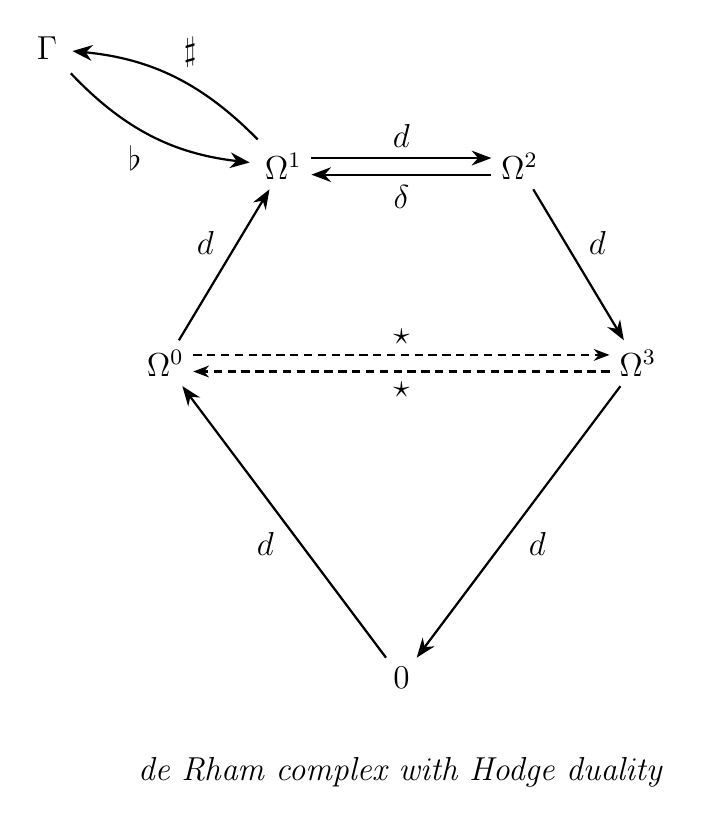
\begin{tikzpicture}[
    node distance=2cm,
    every node/.style={font=\large},
    arrow/.style={-{Stealth[length=2.5mm]}, thick},
    homark/.style={-{Stealth[length=2mm]}, thick, densely dashed},
    parallel shift/.style={transform canvas={yshift=#1}}
]

% === NODES in diamond arrangement ===

% Zero at bottom center
\node (zero) at (0,-4) {$0$};

% Ω⁰ at left
\node (omega0) at (-3, 0) {$\Omega^0$};

% Ω³ at right  
\node (omega3) at (3, 0) {$\Omega^3$};

% $\omega^{1}$ at top-left
\node (omega1) at (-1.5, 2.5) {$\Omega^1$};

% $\omega^{2}$ at top-right
\node (omega2) at (1.5, 2.5) {$\Omega^2$};

% Gamma in upper left corner
\node (Gamma) at (-4.5, 4) {$\Gamma$};

% === DE RHAM COMPLEX (d arrows) ===

% 0 → Ω⁰ 
\draw[arrow] (zero) -- node[midway, below left] {$d$} (omega0);

% Ω⁰ → $\omega^{1}$
\draw[arrow] (omega0) -- node[midway, above left] {$d$} (omega1);

% $\omega^{1}$ → $\omega^{2}$ (parallel pair)
\draw[arrow, parallel shift=3pt] (omega1) -- node[midway, above] {$d$} (omega2);
\draw[arrow, parallel shift=-3pt] (omega2) -- node[midway, below] {$\delta$} (omega1);

% $\omega^{2}$ → Ω³
\draw[arrow] (omega2) -- node[midway, above right] {$d$} (omega3);

% Ω³ → 0
\draw[arrow] (omega3) -- node[midway, below right] {$d$} (zero);

% === HODGE STAR (★) ===

% Ω⁰ $\leftrightarrow$ Ω³ (through center, parallel)
\draw[homark, parallel shift=3pt] (omega0) -- node[midway, above] {$\star$} (omega3);
\draw[homark, parallel shift=-3pt] (omega3) -- node[midway, below] {$\star$} (omega0);

% $\omega^{1}$ $\leftrightarrow$ $\omega^{2}$ already shown with d/δ; ★ is implicit via δ = ★d★

% === MUSICAL ISOMORPHISMS ===

% Use nice curved arrows
\draw[-{Stealth[length=2.5mm, width=2mm]}, thick, shorten >=2pt, shorten <=2pt] 
    (Gamma) to[bend right=20] node[midway, below left] {$\flat$} (omega1);
    
\draw[-{Stealth[length=2.5mm, width=2mm]}, thick, shorten >=2pt, shorten <=2pt] 
    (omega1) to[bend right=20] node[midway, above right] {$\sharp$} (Gamma);

% === LABELS ===
\node at (0, -5.2) {\textit{de Rham complex with Hodge duality}};

\end{tikzpicture}
\end{center}

\vspace{1cm}

% === VERSION 3: Most polished ===

\begin{center}
\textbf{Final Version}
\end{center}

\begin{center}
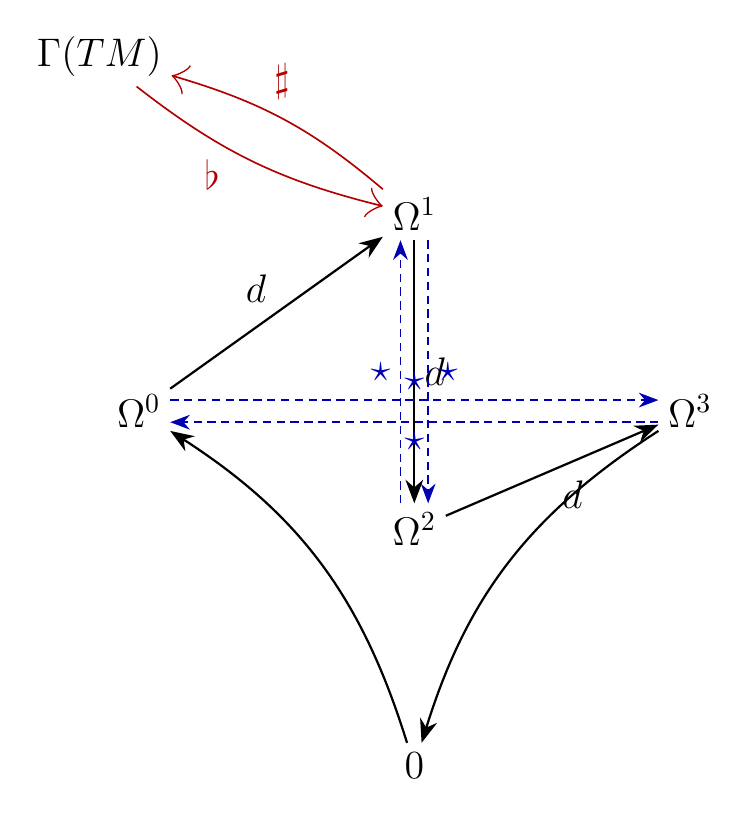
\begin{tikzpicture}[
    every node/.style={font=\Large},
    arrow/.style={-{Stealth[length=3mm]}, line width=0.8pt},
    star/.style={-{Stealth[length=2.5mm]}, line width=0.6pt, densely dashed, blue!70!black},
    musical/.style={-{Classical TikZ Rightarrow[length=2mm]}, line width=0.6pt, red!70!black},
    shift up/.style={transform canvas={yshift=4pt}},
    shift down/.style={transform canvas={yshift=-4pt}}
]

% === NODES ===

% Zero at bottom center
\node (zero) at (0,-4.5) {\Large $0$};

% Diamond arrangement
\node (omega0) at (-3.5, 0) {$\Omega^0$};
\node (omega3) at (3.5, 0) {$\Omega^3$};
\node (omega1) at (0, 2.5) {$\Omega^1$};
\node (omega2) at (0, -1.5) {$\Omega^2$};

% Gamma upper left
\node (Gamma) at (-4, 4.5) {$\Gamma(TM)$};

% === DE RHAM SEQUENCE ===

% 0 → Ω⁰
\draw[arrow] (zero) to[bend right=20] node[midway, left] {$$} (omega0);

% Ω⁰ → $\omega^{1}$  
\draw[arrow] (omega0) -- node[midway, above left] {$d$} (omega1);

% $\omega^{1}$ → $\omega^{2}$ 
\draw[arrow] (omega1) -- node[midway, right] {$d$} (omega2);

% $\omega^{2}$ → Ω³
\draw[arrow] (omega2) -- node[midway, below right] {$d$} (omega3);

% Ω³ → 0
\draw[arrow] (omega3) to[bend right=20] node[midway, right] {$$} (zero);

% === HODGE STAR === 

% Ω⁰ $\leftrightarrow$ Ω³ (horizontal pair through middle)
\draw[star, shift up] (omega0) -- node[midway, above] {$\star$} (omega3);
\draw[star, shift down] (omega3) -- node[midway, below] {$\star$} (omega0);

% $\omega^{1}$ $\leftrightarrow$ $\omega^{2}$ (vertical pair)
\draw[star, transform canvas={xshift=5pt}] (omega1) -- node[midway, right] {$\star$} (omega2);
\draw[star, transform canvas={xshift=-5pt}] (omega2) -- node[midway, left] {$\star$} (omega1);

% === MUSICAL ISOMORPHISMS ===

\draw[musical] (Gamma) to[bend right=12] node[pos=0.4, below left] {$\flat$} (omega1);
\draw[musical] (omega1) to[bend right=12] node[pos=0.6, above right] {$\sharp$} (Gamma);

\end{tikzpicture}
\end{center}

\section{Physical Significance of the $\omega^{2}$-Centric Diagram}

Placing $\omega^{2}$ at the geometric center of the diagram changes our perspective to reveal deep physical significance.

\subsection*{Why $\omega^{2}$ is Central}

\subsubsection*{1. \textbf{Field Strength Lives in $\omega^{2}$}}

In gauge theory, the hierarchy is:
\[
\underbrace{\Omega^0}_{\text{gauge function}} \xrightarrow{d} 
\underbrace{\Omega^1}_{\text{potential } A} \xrightarrow{d} 
\underbrace{\Omega^2}_{\text{field strength } F} \xrightarrow{d} 
\underbrace{\Omega^3}_{\text{Bianchi } dF=0}
\]

The \textbf{physics} (energy, equations of motion, observables) lives at $\omega^{2}$:
\begin{itemize}
	\item Electromagnetic field: $F = dA \in \Omega^2$
	\item Yang-Mills curvature: $F = dA + A \wedge A \in \Omega^2$
	\item Riemann curvature: $R^a{}_b \in \Omega^2(\mathfrak{so}(n))$
\end{itemize}

\subsubsection*{2. \textbf{$\omega^{2}$ is the "Self-Dual" Level (in 4D)}}

In 4 dimensions, the Hodge star satisfies:
\[
\star: \Omega^2 \to \Omega^2, \quad \star^2 = +1 \text{ (Euclidean) or } -1 \text{ (Lorentzian)}
\]

This allows decomposition into \textbf{self-dual} and \textbf{anti-self-dual} parts:
\[
\Omega^2 = \Omega^2_+ \oplus \Omega^2_-
\]

This is central to:
\begin{itemize}
	\item Instantons ($F = \star F$)
	\item Twistor theory
	\item Chiral structure of spinors
	\item Donaldson theory of 4-manifolds
\end{itemize}

\subsubsection*{3. \textbf{Symplectic Structure}}

In Hamiltonian mechanics, everything revolves around $\omega \in \Omega^2(T^*M)$:
\[
\omega = dp_i \wedge dq^i
\]

The symplectic form is a \textbf{closed, non-degenerate 2-form}. Phase space geometry is fundamentally $\omega^{2}$-geometry.

\subsubsection*{4. \textbf{The "Flux" Interpretation}}

\begin{center}
	\begin{tabular}{c|c|c}
		\hline
		\textbf{Form} & \textbf{Integrates over} & \textbf{Physical meaning} \\
		\hline
		$\Omega^0$ & point & field value \\
		$\Omega^1$ & curve & work, circulation \\
		$\boldsymbol{\Omega^2}$ & \textbf{surface} & \textbf{flux} \\
		$\Omega^3$ & volume & total charge/mass \\
		\hline
	\end{tabular}
\end{center}

Flux through surfaces is the natural "middle" concept—it connects local (differential) to global (integral) physics via Stokes' theorem.

\subsubsection*{5. \textbf{In 3D: The Pseudovector Level}}

In 3 dimensions:
\[
\star: \Omega^1 \leftrightarrow \Omega^2
\]

\begin{center}
	\begin{tabular}{c|c}
		\hline
		$\omega^{1}$ (polar vectors) & $\omega^{2}$ (axial vectors) \\
		\hline
		Electric field $\mathbf{E}$ & Magnetic field $\mathbf{B}$ \\
		Velocity $\mathbf{v}$ & Vorticity $\boldsymbol{\omega}$ \\
		Force $\mathbf{F}$ & Torque $\boldsymbol{\tau}$ \\
		Momentum $\mathbf{p}$ & Angular momentum $\mathbf{L}$ \\
		\hline
	\end{tabular}
\end{center}

The $\omega^{1}$ $\leftrightarrow$ $\omega^{2}$ duality is the \textbf{polar/axial} or \textbf{vector/pseudovector} distinction.

\hrulefill

\subsection*{The Diagram's Physical Meaning}

\begin{center}
	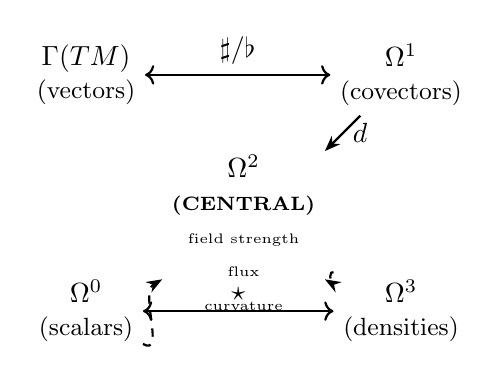
\begin{tikzpicture}[
		node distance=1.2cm,
		every node/.style={font=\normalsize, align=center},
		arrow/.style={-{Stealth[length=2mm]}, thick},
		small node/.style={font=\small}
		]
		
		% Nodes
		\node (GammaTM) at (-2, 3) {$\Gamma(TM)$ \\ \small (vectors)};
		\node (omega1) at (2, 3) {$\Omega^1$ \\ \small (covectors)};
		\node (omega0) at (-2, 0) {$\Omega^0$ \\ \small (scalars)};
		\node (omega3) at (2, 0) {$\Omega^3$ \\ \small (densities)};
		\node (omega2) at (0, 1) {$\Omega^2$ \\ \scriptsize \textbf{(CENTRAL)} \\ \tiny field strength \\ \tiny flux \\ \tiny curvature};
		
		% Musical isomorphisms
		\draw[arrow, <->] (GammaTM) -- node[midway, above] {$\sharp/\flat$} (omega1);
		
		% Exterior derivative
		\draw[arrow] (omega1) -- node[midway, right] {$d$} (omega2);
		
		% Hodge star
		\draw[arrow, <->] (omega0) -- node[midway, above] {$\star$} (omega3);
		\draw[arrow, dashed] (omega0) to[out=-30, in=210] (omega2);
		\draw[arrow, dashed] (omega3) to[out=150, in=-30] (omega2);
		
	\end{tikzpicture}
\end{center}

\textbf{Interpretation:}
\begin{itemize}
	\item $\mathbf{\Omega^0}$ (left): Potentials, scalar fields, gauge functions
	\item $\mathbf{\Omega^3}$ (right): Densities, sources, charges (integrated quantities)
	\item $\mathbf{\Omega^1}$ (top): The "configuration" level—connections, velocities
	\item $\mathbf{\Omega^2}$ (center): The "dynamics" level—field strengths, curvatures, fluxes
	\item $\mathbf{\Gamma(TM)}$ (upper left): Vectors, related to $\omega^{1}$ by the metric via musical isomorphisms
\end{itemize}

The \textbf{musical isomorphisms} ($\flat$ and $\sharp$) require a metric to convert between vectors and covectors. The \textbf{Hodge star} also requires a metric and orientation.


	
\section{The de Rham Complex in Vector Calculus Disguise}

The de Rham complex on $\mathbb{R}^3$, when translated through the metric isomorphisms, becomes:
\begin{equation}
	0 \longrightarrow C^\infty(\mathbb{R}^3) \xrightarrow{\;\mathrm{grad}\;} \mathfrak{X}(\mathbb{R}^3) \xrightarrow{\;\mathrm{curl}\;} \mathfrak{X}(\mathbb{R}^3) \xrightarrow{\;\mathrm{div}\;} C^\infty(\mathbb{R}^3) \longrightarrow 0,
\end{equation}
where $\mathfrak{X}(\mathbb{R}^3)$ denotes vector fields. The identities $\mathrm{curl} \circ \mathrm{grad} = 0$ and $\mathrm{div} \circ \mathrm{curl} = 0$ are the statement that this is a cochain complex.

\begin{figure}[h]
	\centering
	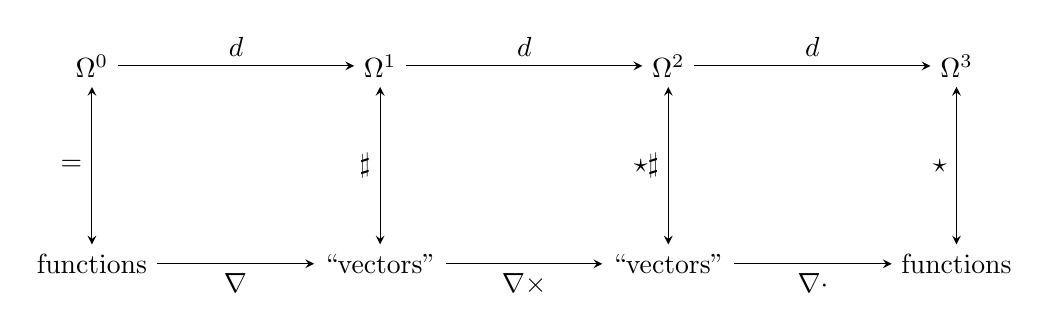
\begin{tikzpicture}[>=stealth, node distance=3cm]
		\node (O0) {$\Omega^0$};
		\node (O1) [right=of O0] {$\Omega^1$};
		\node (O2) [right=of O1] {$\Omega^2$};
		\node (O3) [right=of O2] {$\Omega^3$};
		
		\node (V0) [below=2cm of O0] {functions};
		\node (V1) [below=2cm of O1] {``vectors''};
		\node (V2) [below=2cm of O2] {``vectors''};
		\node (V3) [below=2cm of O3] {functions};
		
		\draw[->] (O0) -- node[above] {$d$} (O1);
		\draw[->] (O1) -- node[above] {$d$} (O2);
		\draw[->] (O2) -- node[above] {$d$} (O3);
		
		\draw[->] (V0) -- node[below] {$\nabla$} (V1);
		\draw[->] (V1) -- node[below] {$\nabla\times$} (V2);
		\draw[->] (V2) -- node[below] {$\nabla\cdot$} (V3);
		
		\draw[<->] (O0) -- node[left] {$=$} (V0);
		\draw[<->] (O1) -- node[left] {$\sharp$} (V1);
		\draw[<->] (O2) -- node[left] {$\star\sharp$} (V2);
		\draw[<->] (O3) -- node[left] {$\star$} (V3);
	\end{tikzpicture}
	\caption{The de Rham complex (top) and its vector calculus disguise (bottom). The vertical arrows are the metric-dependent isomorphisms that obscure the unified structure.}
\end{figure}

\section{Hodge-de Rham for Minkowski Space CL(3,1)}

\begin{center}
	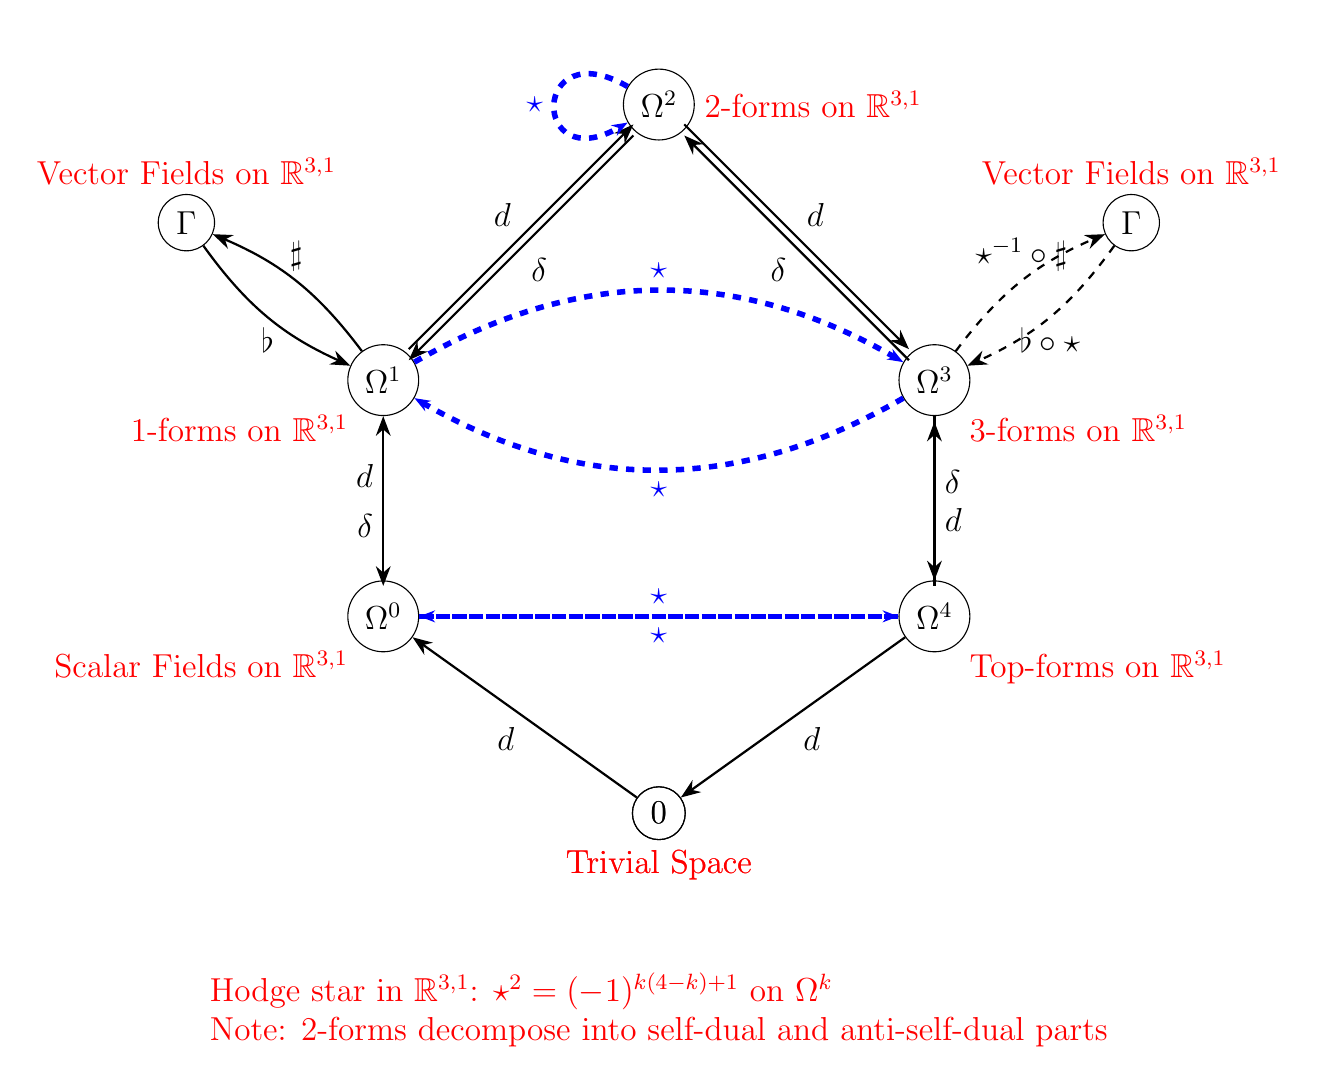
\begin{tikzpicture}[
		node distance=2.5cm and 3cm,
		every node/.style={font=\large},
		arrow/.style={-{Stealth[length=2.5mm]}, thick},
		myarrow/.style={->, blue, thick},
		parallel shift/.style={transform canvas={yshift=#1}},
		hodge/.style={blue, dashed, line width=2pt, -{Stealth[length=2mm]}}
		]
		
		% === NODES ===
		
		% Zero nodes at bottom
		\node [draw, circle,
		label={[text=red]below:Trivial Space}](zero1) at (0,-4) {$0$};
		\node [draw, circle,
		label={[text=red]below:Trivial Space}](zero2) at (0,-4) {$0$};
		
		% First row: Ω⁰ and Ω⁴
		\node [draw, circle,
		label={[text=red]below left:Scalar Fields on $\mathbb{R}^{3,1}$}](omega0) at (-3.5, -1.5) {$\Omega^0$};
		\node [draw, circle,
		label={[text=red]below right:Top-forms on $\mathbb{R}^{3,1}$}] (omega4) at (3.5, -1.5) {$\Omega^4$};
		
		% Second row: Ω¹ and Ω³
		\node [draw, circle,
		label={[text=red]below left:1-forms on $\mathbb{R}^{3,1}$}] (omega1) at (-3.5, 1.5) {$\Omega^1$};
		\node [draw, circle,
		label={[text=red]below right:3-forms on $\mathbb{R}^{3,1}$}](omega3) at (3.5, 1.5) {$\Omega^3$};
		
		% Third row: Ω² (middle)
		\node [draw, circle,
		label={[text=red]right:2-forms on $\mathbb{R}^{3,1}$}] (omega2) at (0, 5) {$\Omega^2$};
		
		% Gamma nodes (vector fields) at edges
		\node [draw, circle,
		label={[text=red]above:Vector Fields on $\mathbb{R}^{3,1}$}] (GammaL) at (-6, 3.5) {$\Gamma$};
		\node [draw, circle,
		label={[text=red]above:Vector Fields on $\mathbb{R}^{3,1}$}] (GammaR) at (6, 3.5) {$\Gamma$};
		
		% === DE RHAM COMPLEX ARROWS (d) ===
		
		% 0 → Ω⁰ and Ω⁴ → 0
		\draw[arrow] (zero1) -- node[midway, below left] {$d$} (omega0);
		\draw[arrow] (omega4) -- node[midway, below right] {$d$} (zero2);
		
		% Ω⁰ → Ω¹
		\draw[arrow] (omega0) -- node[midway, above left] {$d$} (omega1);
		
		% Ω¹ → Ω² (upper left)
		\draw[arrow, parallel shift=2pt] (omega1) -- node[midway, above left] {$d$} (omega2);
		
		% Ω² → Ω³ (upper right)
		\draw[arrow, parallel shift=2pt] (omega2) -- node[midway, above right] {$d$} (omega3);
		
		% Ω³ → Ω⁴
		\draw[arrow] (omega3) -- node[midway, below right] {$d$} (omega4);
		
		% === CODIFFERENTIAL ARROWS (δ) ===
		
		% Ω² → Ω¹ (lower left parallel arrow)
		\draw[arrow, parallel shift=-2pt] (omega2) -- node[midway, below right] {$\delta$} (omega1);
		
		% Ω³ → Ω² (lower right parallel arrow)
		\draw[arrow, parallel shift=-2pt] (omega3) -- node[midway, below left] {$\delta$} (omega2);
		
		% Ω¹ → Ω⁰ (codifferential)
		\draw[arrow, parallel shift=-2pt] (omega1) -- node[midway, below left] {$\delta$} (omega0);
		
		% Ω⁴ → Ω³ (codifferential)
		\draw[arrow, parallel shift=-2pt] (omega4) -- node[midway, above right] {$\delta$} (omega3);
		
		% === HODGE STAR ARROWS (★) FOR MINKOWSKI SPACE ===
		% Note: In Minkowski space, ★² = (-1)^{k(4-k)+1} on k-forms
		
		% Ω⁰ $\leftrightarrow$ Ω⁴ (horizontal, blue dashed)
		\draw[hodge] (omega0) -- node[midway, above] {$\star$} (omega4);
		\draw[hodge] (omega4) -- node[midway, below] {$\star$} (omega0);
		
		% Ω¹ $\leftrightarrow$ Ω³ (curved blue dashed)
		\draw[hodge, bend left=30] (omega1) to node[midway, above] {$\star$} (omega3);
		\draw[hodge, bend left=30] (omega3) to node[midway, below] {$\star$} (omega1);
		
		% Ω² → Ω² (self-dual/anti-self-dual decomposition)
		\draw[hodge, out=150, in=210, looseness=8] 
		(omega2) to node[midway, left] {$\star$} (omega2);
		
		% === MUSICAL ISOMORPHISMS (♭ and ♯) ===
		
		% Left Γ $\leftrightarrow$ Ω¹
		\draw[-{Stealth[length=2.5mm]}, thick, bend right=15] 
		(GammaL) to node[midway, below] {$\flat$} (omega1);
		\draw[-{Stealth[length=2.5mm]}, thick, bend right=15] 
		(omega1) to node[midway, above] {$\sharp$} (GammaL);
		
		% Right Γ $\leftrightarrow$ Ω³ (via Hodge star)
		\draw[-{Stealth[length=2.5mm]}, thick, bend left=15, dashed] 
		(GammaR) to node[midway, below] {$\flat \circ \star$} (omega3);
		\draw[-{Stealth[length=2.5mm]}, thick, bend left=15, dashed] 
		(omega3) to node[midway, above] {$\star^{-1} \circ \sharp$} (GammaR);
		% === ADDITIONAL NOTES ===
		\node[text=red, align=left] at (0, -6.5) {
			Hodge star in $\mathbb{R}^{3,1}$: $\star^2 = (-1)^{k(4-k)+1}$ on $\Omega^k$\\
			Note: 2-forms decompose into self-dual and anti-self-dual parts
		};
		
	\end{tikzpicture}
\end{center}


\begin{center}
	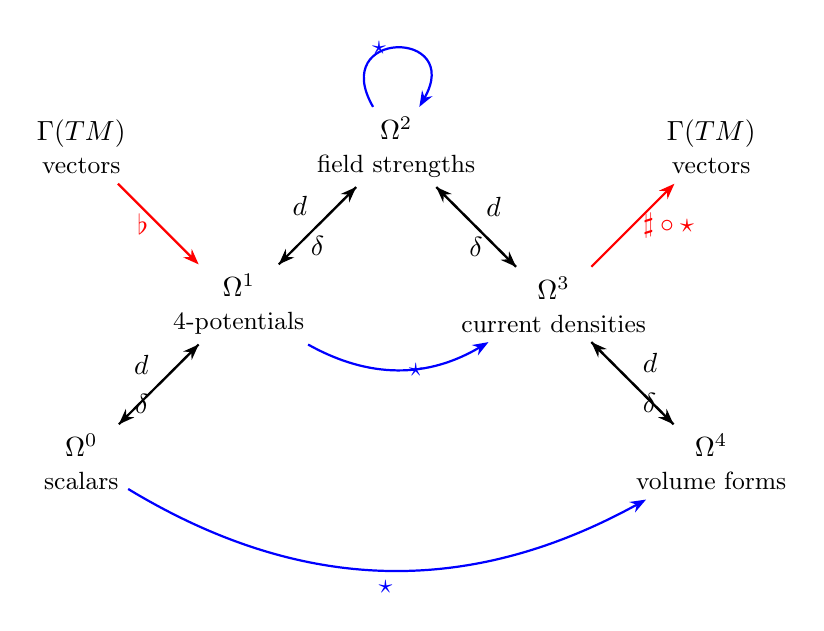
\begin{tikzpicture}[
		node distance=1.5cm,
		every node/.style={font=\normalsize, align=center},
		arrow/.style={-{Stealth[length=2mm]}, thick},
		small node/.style={font=\small}
		]
		
		% Nodes
		\node (omega0) at (-4, 0) {$\Omega^0$ \\ \small scalars};
		\node (omega1) at (-2, 2) {$\Omega^1$ \\ \small 4-potentials};
		\node (omega2) at (0, 4) {$\Omega^2$ \\ \small field strengths};
		\node (omega3) at (2, 2) {$\Omega^3$ \\ \small current densities};
		\node (omega4) at (4, 0) {$\Omega^4$ \\ \small volume forms};
		
		\node (GammaL) at (-4, 4) {$\Gamma(TM)$ \\ \small vectors};
		\node (GammaR) at (4, 4) {$\Gamma(TM)$ \\ \small vectors};
		
		% de Rham complex
		\draw[arrow] (omega0) -- node[midway, above left] {$d$} (omega1);
		\draw[arrow] (omega1) -- node[midway, above left] {$d$} (omega2);
		\draw[arrow] (omega2) -- node[midway, above right] {$d$} (omega3);
		\draw[arrow] (omega3) -- node[midway, above right] {$d$} (omega4);
		
		% Codifferential
		\draw[arrow, dashed] (omega1) -- node[midway, below left] {$\delta$} (omega0);
		\draw[arrow, dashed] (omega2) -- node[midway, below] {$\delta$} (omega1);
		\draw[arrow, dashed] (omega3) -- node[midway, below] {$\delta$} (omega2);
		\draw[arrow, dashed] (omega4) -- node[midway, below right] {$\delta$} (omega3);
		
		% Hodge star
		\draw[arrow, blue] (omega0) to[bend right=30] node[midway, below] {$\star$} (omega4);
		\draw[arrow, blue] (omega1) to[bend right=30] node[midway, right] {$\star$} (omega3);
		\draw[arrow, blue] (omega2) to[out=120, in=60, looseness=5] node[midway, left] {$\star$} (omega2);
		
		% Musical isomorphisms
		\draw[arrow, red] (GammaL) -- node[midway, left] {$\flat$} (omega1);
		\draw[arrow, red] (omega3) -- node[midway, right] {$\sharp \circ \star$} (GammaR);
		
	\end{tikzpicture}
\end{center}

Physical Interpretation of the Minkowski Form Degrees

\begin{enumerate}

\item $\mathbf{\Omega^0}$: Scalar Fields
- Higgs field $\phi(x)$ in electroweak theory
- Dilaton field in string theory
- Conformal factors in general relativity

\item $\mathbf{\Omega^1}$: 4-Potentials (Central in Gauge Theory)
- Electromagnetic potential: $A = A_\mu dx^\mu$
- Connection 1-forms in gauge theories: $A = A_\mu^a T_a dx^\mu$
- Gravitational tetrad (coframe): $e^a = e^a_\mu dx^\mu$

\item $\mathbf{\Omega^2}$: Field Strengths (The Dynamics)
- Electromagnetic field: $F = dA = \frac{1}{2}F_{\mu\nu}dx^\mu \wedge dx^\nu$
- Yang-Mills curvature: $F = dA + A \wedge A$
- Riemann curvature 2-form: $R^a_{\ b} = d\omega^a_{\ b} + \omega^a_{\ c} \wedge \omega^c_{\ b}$
- Torsion 2-form: $T^a = de^a + \omega^a_{\ b} \wedge e^b$

\item $\mathbf{\Omega^3}$: Currents and Sources
- Electromagnetic current 3-form: $J = \star j$ where $j = j_\mu dx^\mu$
- Stress-energy current: $\mathcal{T}^a = \star T^a$ (tetrad formulation)
- Topological current densities

\item $\mathbf{\Omega^4}$: Lagrangians and Topological Terms
- Volume form: $\text{vol}_4 = \sqrt{|g|}d^4x$
- Lagrangian densities: $\mathcal{L}\text{vol}_4$
- Pontryagin and Euler density forms

\item The Hodge Star in Minkowski Space: A Physical Perspective

The Hodge star operator in $\mathbb{R}^{3,1}$ satisfies:
\[
\star^2 = (-1)^{k(4-k)+1} \ \text{on} \ \Omega^k
\]

This leads to crucial physical distinctions:

\item For $\mathbf{\Omega^2}$: Self-Dual/Anti-Self-Dual Decomposition
Since $\star^2 = -1$ on 2-forms, we can define complex self-dual and anti-self-dual parts:
\[
F_{\pm} = \frac{1}{2}(F \mp i\star F)
\]
with $\star F_{\pm} = \pm i F_{\pm}$. This decomposition is fundamental to:
- Instantons in Yang-Mills theory ($F = \star F$ becomes $F_- = 0$)
- Twistor theory and the Penrose transform
- Chiral representations of the Lorentz group
- Maxwell's equations in vacuum: $dF = 0$ and $d\star F = 0$ imply $dF_{\pm} = 0$

\item For $\mathbf{\Omega^1 \leftrightarrow \Omega^3}$: Potential-Current Duality
The isomorphism $\Omega^1 \leftrightarrow \Omega^3$ via $\star$ encodes:
- Electric-magnetic duality: $A \leftrightarrow \star F$
- Hodge decomposition: Any 1-form $A$ can be written as $A = d\phi + \delta B + \text{harmonic}$
- Lorenz gauge condition: $\delta A = 0$ becomes $d\star A = 0$

\item From Forms to General Relativity: The Dictionary

The form language provides a coordinate-free formulation of general relativity:

\item The Tetrad Formalism
Instead of the metric tensor $g_{\mu\nu}$, we use:
- Tetrad (vierbein): $e^a = e^a_\mu dx^\mu \in \Omega^1$ (four 1-forms)
- Metric: $g = \eta_{ab} e^a \otimes e^b$
- Spin connection: $\omega^{ab} = \omega^{ab}_\mu dx^\mu \in \Omega^1(\mathfrak{so}(3,1))$

\item Cartan Structure Equations
The fundamental equations become:
\begin{align*}
	\text{First structure equation:} & \quad T^a = de^a + \omega^a_{\ b} \wedge e^b \in \Omega^2 \\
	\text{Second structure equation:} & \quad R^a_{\ b} = d\omega^a_{\ b} + \omega^a_{\ c} \wedge \omega^c_{\ b} \in \Omega^2
\end{align*}

\item The Einstein-Hilbert Action
In form language:
\[
S_{\text{EH}} = \frac{1}{16\pi G} \int \epsilon_{abcd} R^{ab} \wedge e^c \wedge e^d
\]
where $\epsilon_{abcd}$ is the Levi-Civita symbol.

\item Bianchi Identities
The geometric identities become simple statements in the de Rham complex:
\[
dR^a_{\ b} + \omega^a_{\ c} \wedge R^c_{\ b} - R^a_{\ c} \wedge \omega^c_{\ b} = 0
\]
This is the form version of $\nabla_{[\mu}R_{\nu\rho]\sigma}^{\ \ \ \ \lambda} = 0$.

\item The de Rham Complex in Relativistic Physics

\item Maxwell's Equations (Form Version)
\begin{align*}
	dF &= 0 \quad &\text{(Homogeneous: } \nabla \cdot \mathbf{B} = 0, \ \nabla \times \mathbf{E} + \frac{\partial \mathbf{B}}{\partial t} = 0\text{)} \\
	d\star F &= J \quad &\text{(Inhomogeneous: } \nabla \cdot \mathbf{E} = \rho, \ \nabla \times \mathbf{B} - \frac{\partial \mathbf{E}}{\partial t} = \mathbf{j}\text{)}
\end{align*}
where $F \in \Omega^2$, $J \in \Omega^3$, and $\star$ is the Hodge star of Minkowski space.

\item Einstein's Equations (Form Version)
\[
\frac{1}{2}\epsilon_{abcd} R^{bc} \wedge e^d = 8\pi G \star \mathcal{T}_a
\]
where $\mathcal{T}_a \in \Omega^3$ is the stress-energy 3-form.

\item Gauge Theories
For a gauge group $G$ with Lie algebra $\mathfrak{g}$:
- Potential: $A \in \Omega^1(\mathfrak{g})$
- Field strength: $F = dA + A \wedge A \in \Omega^2(\mathfrak{g})$
- Yang-Mills equation: $d_A \star F = \star J$ where $d_A = d + [A, \cdot]$

\item Musical Isomorphisms: Raising and Lowering Indices

The musical isomorphisms $\flat$ and $\sharp$ in the diagram correspond precisely to index manipulation in tensor calculus:

- $\flat: \Gamma(TM) \to \Omega^1$: $v^\mu \mapsto v_\mu = g_{\mu\nu}v^\nu$
- $\sharp: \Omega^1 \to \Gamma(TM)$: $\omega_\mu \mapsto \omega^\mu = g^{\mu\nu}\omega_\nu$

The additional isomorphisms $\Gamma(TM) \leftrightarrow \Omega^3$ via $\star$ represent:
- Vector density $\leftrightarrow$ 3-form correspondence
- Current vectors $\leftrightarrow$ Current 3-forms: $j^\mu \leftrightarrow J = \star j$
- Killing vectors $\leftrightarrow$ Killing-Yano tensors

\item Physical Significance of the Center: $\mathbf{\Omega^2}$

Just as in the $\mathbb{R}^3$ case, $\Omega^2$ occupies a central position in Minkowski space:

1. Field Strength Centrality: All fundamental forces (electromagnetic, weak, strong, gravitational) are described by curvature 2-forms.

2. Self-Duality Structure: The property $\star^2 = -1$ on $\Omega^2$ leads to the complex structure essential for:
- Spinor representations via the isomorphism $\Omega^2 \cong \mathfrak{so}(3,1) \otimes \mathbb{C}$
- Twistor theory where null 2-forms correspond to twistors
- Instantons and monopoles as self-dual/anti-self-dual solutions

3. Bianchi Identities as Conservation Laws: 
- Maxwell: $dF = 0$ (conservation of magnetic flux)
- Einstein: $d_\omega R = 0$ (differential Bianchi identity → stress-energy conservation)

4. Duality Transformations: Electric-magnetic duality $F \leftrightarrow \star F$ is a rotation in the space of 2-forms.

\item The de Rham Complex and Conservation Laws

The sequence:
\[
0 \longrightarrow \Omega^0 \xrightarrow{d} \Omega^1 \xrightarrow{d} \Omega^2 \xrightarrow{d} \Omega^3 \xrightarrow{d} \Omega^4 \longrightarrow 0
\]

encodes a hierarchy of conservation laws:

- $d^2 = 0$: Poincaré lemma and the existence of potentials
- $\delta^2 = 0$: Adjoint conservation laws
- Hodge decomposition: $\Omega^k = d\Omega^{k-1} \oplus \delta\Omega^{k+1} \oplus \mathcal{H}^k$
where $\mathcal{H}^k$ are harmonic forms (solutions of $d\omega = 0$ and $\delta\omega = 0$)

In physical terms:
- Exact forms ($\omega = d\alpha$): "pure gauge" configurations
- Coexact forms ($\omega = \delta\beta$): sourced fields
- Harmonic forms: vacuum solutions, zero modes, topological sectors

\item Conclusion

The Hodge-deRham complex on Minkowski space $\mathbb{R}^{3,1}$ provides a unified geometric framework that reveals the deep connections between:
- Differential topology (de Rham cohomology)
- Riemannian/Lorentzian geometry (Hodge theory)
- Gauge theories (fiber bundles and connections)
- General relativity (Cartan geometry)

The diagram is not merely an algebraic curiosity but a map of the conceptual landscape of modern theoretical physics, showing how different physical concepts are interrelated through the fundamental operations of exterior calculus. The central role of $\Omega^2$ reflects the fact that dynamics (field strengths, curvatures) mediate between potentials ($\Omega^1$) and sources ($\Omega^3$), with the Hodge star providing the crucial duality transformations that underlie symmetry principles like electric-magnetic duality.

This formulation transcends coordinate-dependent descriptions and reveals the intrinsic geometric nature of physical laws—a perspective that becomes essential when extending these ideas to curved spacetimes, quantum gravity, and beyond.
\end{enumerate}



\section{Hodge-de Rham Complex for the Octonions: CL(0,7)}

\begin{center}
	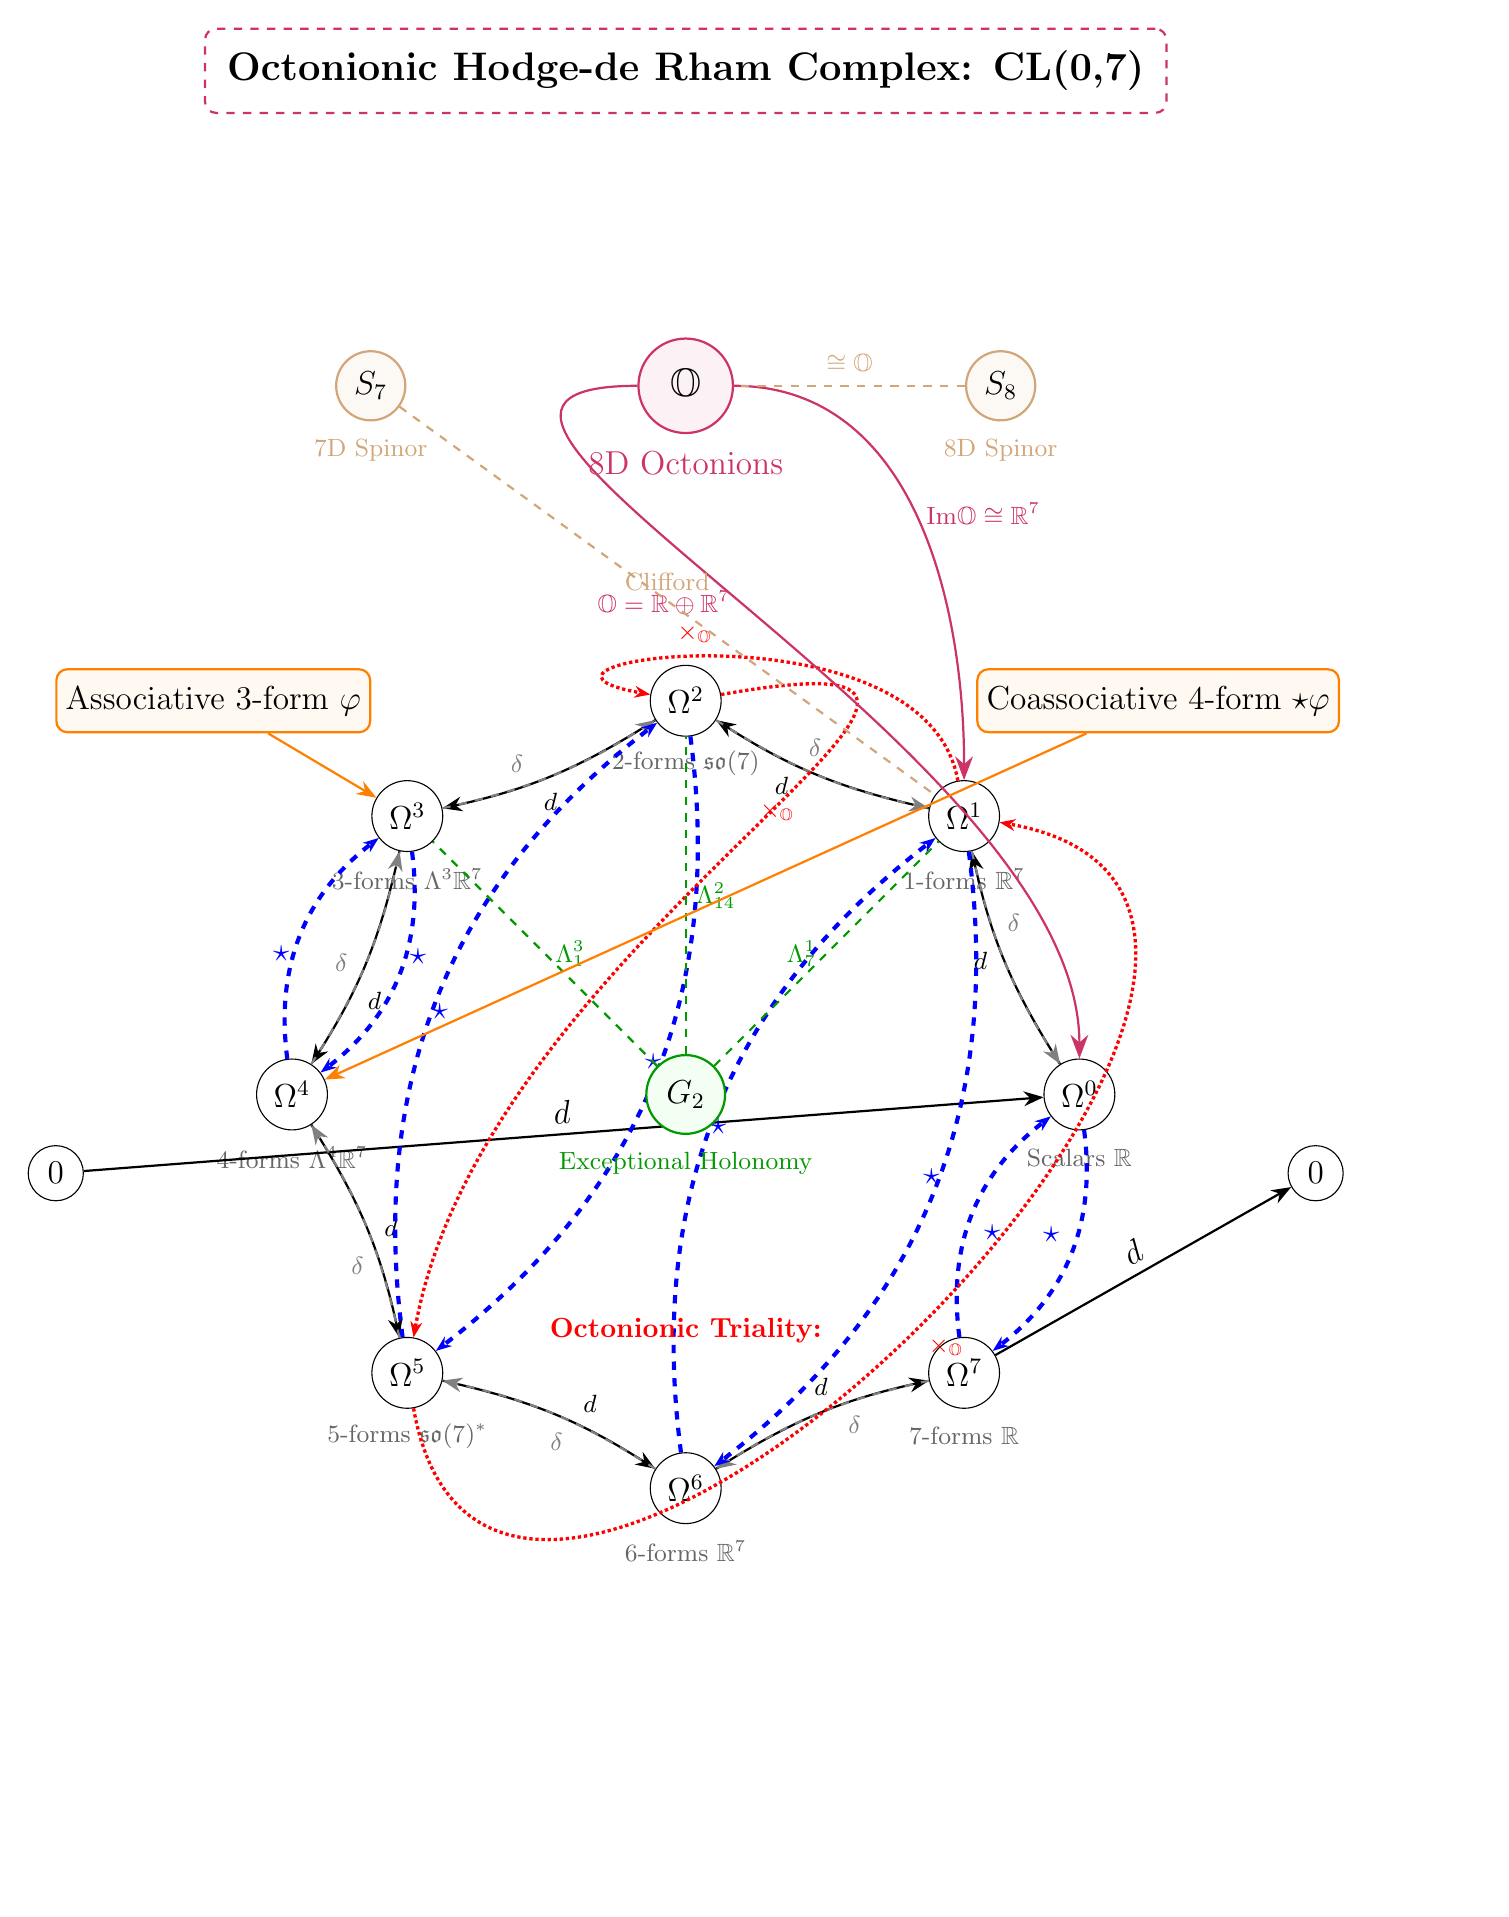
\begin{tikzpicture}[
		node distance=2.5cm and 3cm,
		every node/.style={font=\large},
		arrow/.style={-{Stealth[length=2.5mm]}, thick},
		hodge/.style={blue, dashed, line width=1.5pt, -{Stealth[length=2mm]}},
		triality/.style={red, densely dotted, line width=1.2pt, -{Stealth[length=2mm]}},
		parallel shift/.style={transform canvas={yshift=#1}},
		octonion/.style={draw=purple!80, thick, dashed, rectangle, rounded corners, inner sep=8pt}
		]
		
		% === TITLE ===
		\node[octonion] at (0, 13) {\Large \textbf{Octonionic Hodge-de Rham Complex: CL(0,7)}};
		
		% === ZERO NODES ===
		\node[draw, circle, minimum size=0.7cm] (zero0) at (-8, -1) {$0$};
		\node[draw, circle, minimum size=0.7cm] (zero7) at (8, -1) {$0$};
		
		% === OCTONION NODE ===
		\node[draw=purple!80, thick, circle, minimum size=1.2cm, fill=purple!5] 
		(octonions) at (0, 9) {\Large $\mathbb{O}$};
		\node[text=purple!80, below=0.1cm of octonions] {8D Octonions};
		
		% === FORM SPACES IN A CIRCLE ARRANGEMENT ===
		
		% Calculate positions on a circle
		\foreach \i/\deg/\name/\labeltext in {0/0/omega0/{Scalars $\mathbb{R}$},
			1/45/omega1/{1-forms $\mathbb{R}^7$},
			2/90/omega2/{2-forms $\mathfrak{so}(7)$},
			3/135/omega3/{3-forms $\Lambda^3\mathbb{R}^7$},
			4/180/omega4/{4-forms $\Lambda^4\mathbb{R}^7$},
			5/225/omega5/{5-forms $\mathfrak{so}(7)^*$},
			6/270/omega6/{6-forms $\mathbb{R}^7$},
			7/315/omega7/{7-forms $\mathbb{R}$}} {
			\pgfmathsetmacro{\radius}{5}
			\pgfmathsetmacro{\x}{\radius*cos(\deg)}
			\pgfmathsetmacro{\y}{\radius*sin(\deg)}
			\node[draw, circle, minimum size=0.8cm] (\name) at (\x, \y) {$\Omega^{\i}$};
			\node[text=black!60, font=\small] at (\x, \y-0.8) {\labeltext};
		}
		
		% === DE RHAM COMPLEX ARROWS (d) - Outer circle ===
		\foreach \i/\j in {0/1, 1/2, 2/3, 3/4, 4/5, 5/6, 6/7} {
			\draw[arrow] (omega\i) to[bend left=10] node[midway, auto, pos=0.6, font=\small] {$d$} (omega\j);
		}
		
		% 0 → Ω⁰ and Ω⁷ → 0
		\draw[arrow] (zero0) -- node[midway, above, sloped] {$d$} (omega0);
		\draw[arrow] (omega7) -- node[midway, above, sloped] {$d$} (zero7);
		
		% === CODIFFERENTIAL ARROWS (δ) - Inner circle ===
		\foreach \i/\j in {1/0, 2/1, 3/2, 4/3, 5/4, 6/5, 7/6} {
			\draw[arrow, dashed, gray] (omega\i) to[bend right=10] node[midway, auto, pos=0.4, font=\small] {$\delta$} (omega\j);
		}
		
		% === HODGE STAR ARROWS (★) ===
		% CL(0,7): Negative definite metric in 7D: ★² = (-1)^{k(7-k)}
		\draw[hodge] (omega0) to[bend left=30] node[midway, above left] {$\star$} (omega7);
		\draw[hodge] (omega7) to[bend left=30] node[midway, below right] {$\star$} (omega0);
		
		\draw[hodge] (omega1) to[bend left=30] node[midway, above] {$\star$} (omega6);
		\draw[hodge] (omega6) to[bend left=30] node[midway, below] {$\star$} (omega1);
		
		\draw[hodge] (omega2) to[bend left=30] node[midway, above] {$\star$} (omega5);
		\draw[hodge] (omega5) to[bend left=30] node[midway, below] {$\star$} (omega2);
		
		\draw[hodge] (omega3) to[bend left=30] node[midway, above right] {$\star$} (omega4);
		\draw[hodge] (omega4) to[bend left=30] node[midway, below left] {$\star$} (omega3);
		
		% === TRIALITY ARROWS - Special octonionic isomorphisms ===
		\node[text=red, font=\bfseries] at (0, -3) {Octonionic Triality:};
		
		% Ω¹ $\leftrightarrow$ Ω² $\leftrightarrow$ Ω⁵ connections via octonion multiplication
		\draw[triality] (omega1) to[out=100, in=170, looseness=1.5] 
		node[midway, above left, font=\small] {$\times_{\mathbb{O}}$} (omega2);
		\draw[triality] (omega2) to[out=10, in=80, looseness=1.5] 
		node[midway, above right, font=\small] {$\times_{\mathbb{O}}$} (omega5);
		\draw[triality] (omega5) to[out=-80, in=-10, looseness=1.5] 
		node[midway, below right, font=\small] {$\times_{\mathbb{O}}$} (omega1);
		
		% === OCTONION TO FORM SPACES CONNECTIONS ===
		% Octonions decompose as 1 + 7
		\draw[purple!80, thick, -{Stealth[length=3mm]}] 
		(octonions) to[out=180, in=90] node[midway, left, font=\small] {$\mathbb{O} = \mathbb{R} \oplus \mathbb{R}^7$} (omega0);
		\draw[purple!80, thick, -{Stealth[length=3mm]}] 
		(octonions) to[out=0, in=90] node[midway, right, font=\small] {Im$\mathbb{O} \cong \mathbb{R}^7$} (omega1);
		
		% === G₂ HOLONOMY SPHERE ===
		\node[draw=green!60!black, thick, circle, minimum size=1cm, fill=green!5] 
		(g2) at (0, 0) {$G_2$};
		\node[text=green!60!black, below=0.1cm of g2, font=\small] {Exceptional Holonomy};
		
		% G₂ acts on Ω¹, Ω², Ω³ in special ways
		\draw[green!60!black, thick, dashed] (g2) -- node[midway, left, font=\small] {$\Lambda^1_7$} (omega1);
		\draw[green!60!black, thick, dashed] (g2) -- node[midway, right, font=\small] {$\Lambda^2_{14}$} (omega2);
		\draw[green!60!black, thick, dashed] (g2) -- node[midway, right, font=\small] {$\Lambda^3_1$} (omega3);
		
		% === SPECIAL 3-FORM AND 4-FORM ===
		\node[draw=orange, thick, rectangle, rounded corners, minimum width=2cm, minimum height=0.8cm, fill=orange!5] 
		(associative) at (-6, 5) {Associative 3-form $\varphi$};
		\node[draw=orange, thick, rectangle, rounded corners, minimum width=2cm, minimum height=0.8cm, fill=orange!5] 
		(coassociative) at (6, 5) {Coassociative 4-form $\star\varphi$};
		
		\draw[orange, thick, -{Stealth[length=2.5mm]}] (associative) -- (omega3);
		\draw[orange, thick, -{Stealth[length=2.5mm]}] (coassociative) -- (omega4);
		
		% === SPINOR CONNECTIONS ===
		\node[draw=brown!70, thick, circle, minimum size=0.8cm, fill=brown!5] 
		(spinor7) at (-4, 9) {$S_7$};
		\node[draw=brown!70, thick, circle, minimum size=0.8cm, fill=brown!5] 
		(spinor8) at (4, 9) {$S_8$};
		\node[text=brown!70, below=0.1cm of spinor7, font=\small] {7D Spinor};
		\node[text=brown!70, below=0.1cm of spinor8, font=\small] {8D Spinor};
		
		% Spinor to form connections
		\draw[brown!70, thick, dashed] (spinor7) -- node[midway, above, font=\small] {Clifford} (omega1);
		\draw[brown!70, thick, dashed] (spinor8) -- node[midway, above, font=\small] {$\cong \mathbb{O}$} (octonions);
		
	\end{tikzpicture}
\end{center}


\section{ CL(0,7)}

\begin{center}
	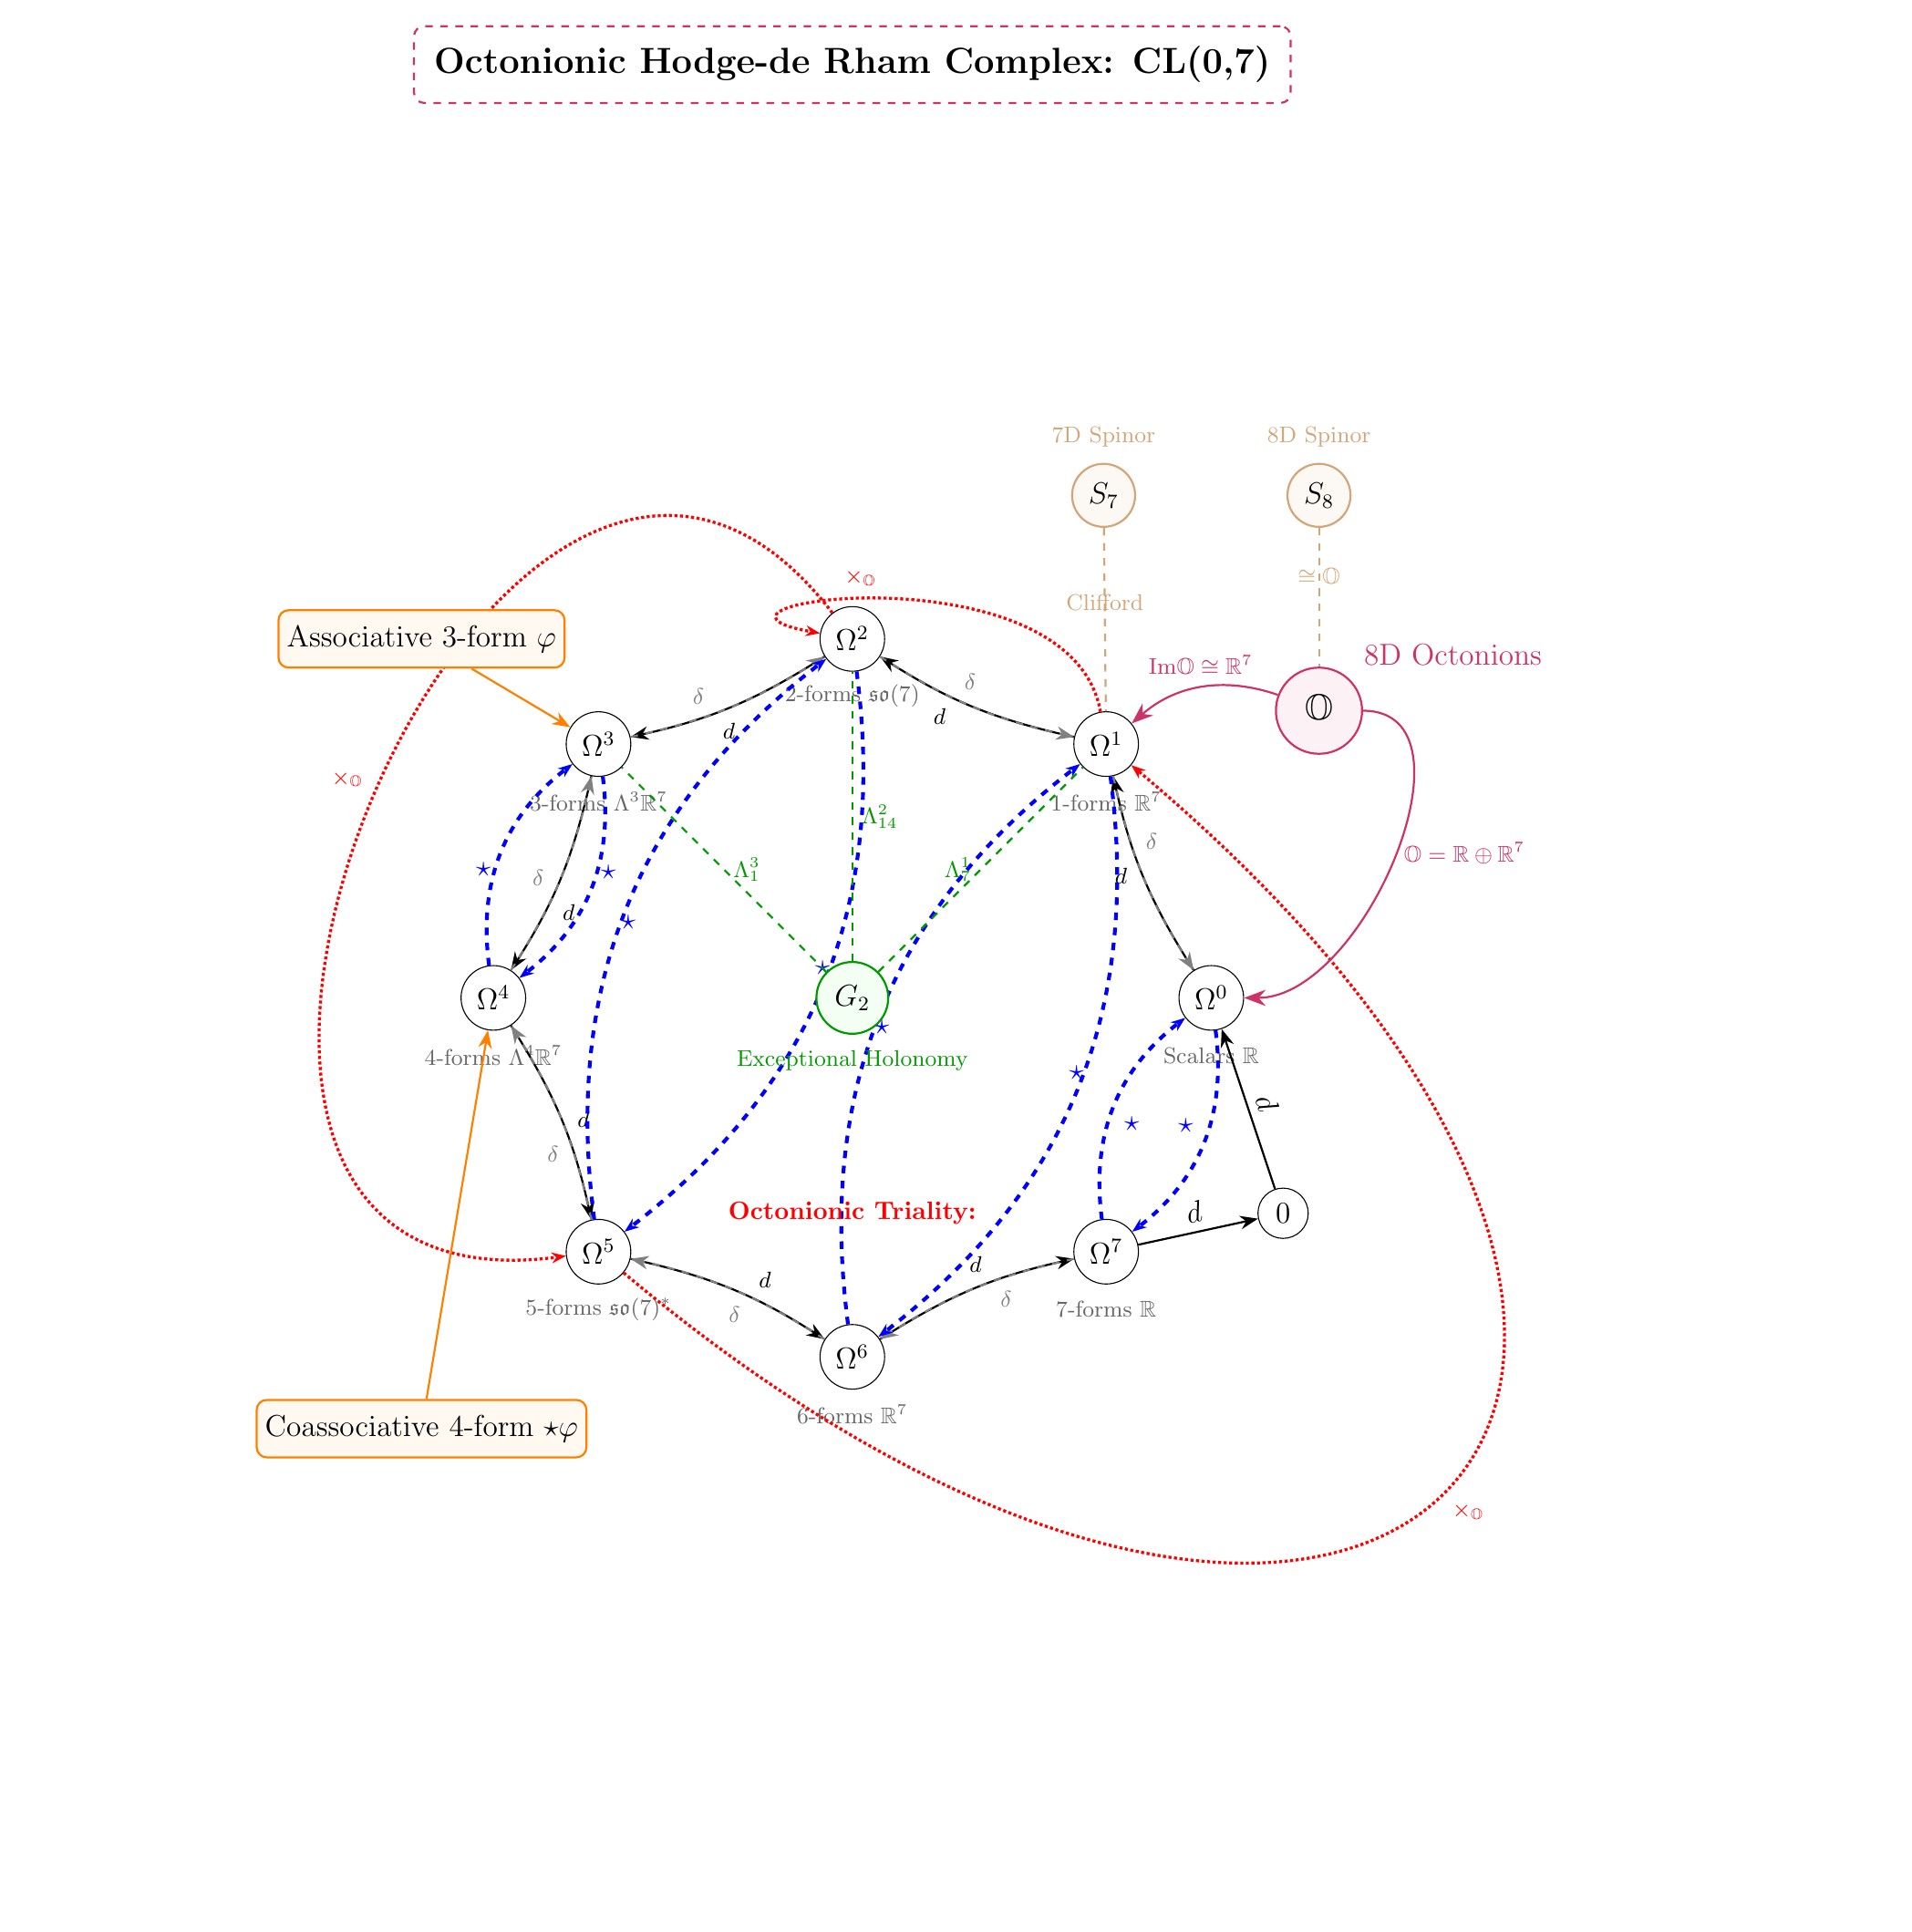
\begin{tikzpicture}[
		node distance=2.5cm and 3cm,
		every node/.style={font=\large},
		arrow/.style={-{Stealth[length=2.5mm]}, thick},
		hodge/.style={blue, dashed, line width=1.5pt, -{Stealth[length=2mm]}},
		triality/.style={red, densely dotted, line width=1.2pt, -{Stealth[length=2mm]}},
		parallel shift/.style={transform canvas={yshift=#1}},
		octonion/.style={draw=purple!80, thick, dashed, rectangle, rounded corners, inner sep=8pt}
		]
		
		% === TITLE ===
		\node[octonion] at (0, 13) {\Large \textbf{Octonionic Hodge-de Rham Complex: CL(0,7)}};
		
		% === ZERO NODES ===
		%\node[draw, circle, minimum size=0.7cm] (zero0) at (-8, -1) {$0$};
		\node[draw, circle, minimum size=0.7cm] (zero7) at (6, -3) {$0$};
		
		% === OCTONION NODE ===
		\node[draw=purple!80, thick, circle, minimum size=1.2cm, fill=purple!5] 
		(octonions) at (6.5, 4) {\Large $\mathbb{O}$};
		\node[text=purple!80, above right=0.1cm of octonions] {8D Octonions};
		
		% === FORM SPACES IN A CIRCLE ARRANGEMENT ===
		
		% Calculate positions on a circle
		\foreach \i/\deg/\name/\labeltext in {0/0/omega0/{Scalars $\mathbb{R}$},
			1/45/omega1/{1-forms $\mathbb{R}^7$},
			2/90/omega2/{2-forms $\mathfrak{so}(7)$},
			3/135/omega3/{3-forms $\Lambda^3\mathbb{R}^7$},
			4/180/omega4/{4-forms $\Lambda^4\mathbb{R}^7$},
			5/225/omega5/{5-forms $\mathfrak{so}(7)^*$},
			6/270/omega6/{6-forms $\mathbb{R}^7$},
			7/315/omega7/{7-forms $\mathbb{R}$}} {
			\pgfmathsetmacro{\radius}{5}
			\pgfmathsetmacro{\x}{\radius*cos(\deg)}
			\pgfmathsetmacro{\y}{\radius*sin(\deg)}
			\node[draw, circle, minimum size=0.8cm] (\name) at (\x, \y) {$\Omega^{\i}$};
			\node[text=black!60, font=\small] at (\x, \y-0.8) {\labeltext};
		}
		
		% === DE RHAM COMPLEX ARROWS (d) - Outer circle ===
		\foreach \i/\j in {0/1, 1/2, 2/3, 3/4, 4/5, 5/6, 6/7} {
			\draw[arrow] (omega\i) to[bend left=10] node[midway, auto, pos=0.6, font=\small] {$d$} (omega\j);
		}
		
		% 0 → Ω⁰ and Ω⁷ → 0
		\draw[arrow] (zero7) -- node[midway, above, sloped] {$d$} (omega0);
		\draw[arrow] (omega7) -- node[midway, above, sloped] {$d$} (zero7);
		
		% === CODIFFERENTIAL ARROWS (δ) - Inner circle ===
		\foreach \i/\j in {1/0, 2/1, 3/2, 4/3, 5/4, 6/5, 7/6} {
			\draw[arrow, dashed, gray] (omega\i) to[bend right=10] node[midway, auto, pos=0.4, font=\small] {$\delta$} (omega\j);
		}
		
		% === HODGE STAR ARROWS (★) ===
		% CL(0,7): Negative definite metric in 7D: ★² = (-1)^{k(7-k)}
		\draw[hodge] (omega0) to[bend left=30] node[midway, above left] {$\star$} (omega7);
		\draw[hodge] (omega7) to[bend left=30] node[midway, below right] {$\star$} (omega0);
		
		\draw[hodge] (omega1) to[bend left=30] node[midway, above] {$\star$} (omega6);
		\draw[hodge] (omega6) to[bend left=30] node[midway, below] {$\star$} (omega1);
		
		\draw[hodge] (omega2) to[bend left=30] node[midway, above] {$\star$} (omega5);
		\draw[hodge] (omega5) to[bend left=30] node[midway, below] {$\star$} (omega2);
		
		\draw[hodge] (omega3) to[bend left=30] node[midway, above right] {$\star$} (omega4);
		\draw[hodge] (omega4) to[bend left=30] node[midway, below left] {$\star$} (omega3);
		
		% === TRIALITY ARROWS - Special octonionic isomorphisms ===
		\node[text=red, font=\bfseries] at (0, -3) {Octonionic Triality:};
		
		% Ω¹ $\leftrightarrow$ Ω² $\leftrightarrow$ Ω⁵ connections via octonion multiplication
		% The red dashed lines that need cleaing up
		\draw[triality] (omega1) to[out=100, in=170, looseness=1.5] 
		node[midway, above left, font=\small] {$\times_{\mathbb{O}}$} (omega2);
		\draw[triality] (omega2) to[bend right=120, looseness=2] 
		node[midway, above left, font=\small] {$\times_{\mathbb{O}}$} (omega5);
		\draw[triality] (omega5) to[out=-40, in=-40, looseness=3.5] 
		node[midway, below right, font=\small] {$\times_{\mathbb{O}}$} (omega1);
		
		% === OCTONION TO FORM SPACES CONNECTIONS ===
		% Octonions decompose as 1 + 7
		\draw[purple!80, thick, -{Stealth[length=3mm]}] 
		(octonions) to[out=0, in=0] node[midway, right, font=\small] {$\mathbb{O} = \mathbb{R} \oplus \mathbb{R}^7$} (omega0);
		\draw[purple!80, thick, -{Stealth[length=3mm]}] 
		(octonions) to[bend right=30] node[midway, above, font=\small] {Im$\mathbb{O} \cong \mathbb{R}^7$} (omega1);
		
		% === G₂ HOLONOMY SPHERE ===
		\node[draw=green!60!black, thick, circle, minimum size=1cm, fill=green!5] 
		(g2) at (0, 0) {$G_2$};
		\node[text=green!60!black, below=0.1cm of g2, font=\small] {Exceptional Holonomy};
		
		% G₂ acts on Ω¹, Ω², Ω³ in special ways
		\draw[green!60!black, thick, dashed] (g2) -- node[midway, left, font=\small] {$\Lambda^1_7$} (omega1);
		\draw[green!60!black, thick, dashed] (g2) -- node[midway, right, font=\small] {$\Lambda^2_{14}$} (omega2);
		\draw[green!60!black, thick, dashed] (g2) -- node[midway, right, font=\small] {$\Lambda^3_1$} (omega3);
		
		% === SPECIAL 3-FORM AND 4-FORM ===
		\node[draw=orange, thick, rectangle, rounded corners, minimum width=2cm, minimum height=0.8cm, fill=orange!5] 
		(associative) at (-6, 5) {Associative 3-form $\varphi$};
		\node[draw=orange, thick, rectangle, rounded corners, minimum width=2cm, minimum height=0.8cm, fill=orange!5] 
		(coassociative) at (-6, -6) {Coassociative 4-form $\star\varphi$};
		
		\draw[orange, thick, -{Stealth[length=2.5mm]}] (associative) -- (omega3);
		\draw[orange, thick, -{Stealth[length=2.5mm]}] (coassociative) -- (omega4);
		
		% === SPINOR CONNECTIONS ===
		\node[draw=brown!70, thick, circle, minimum size=0.8cm, fill=brown!5] 
		(spinor7) at (3.5, 7) {$S_7$};
		\node[draw=brown!70, thick, circle, minimum size=0.8cm, fill=brown!5] 
		(spinor8) at (6.5, 7) {$S_8$};
		\node[text=brown!70, above=0.1cm of spinor7, font=\small] {7D Spinor};
		\node[text=brown!70, above=0.1cm of spinor8, font=\small] {8D Spinor};
		
		% Spinor to form connections
		\draw[brown!70, thick, dashed] (spinor7) -- node[midway, above, font=\small] {Clifford} (omega1);
		\draw[brown!70, thick, dashed] (spinor8) -- node[midway, above, font=\small] {$\cong \mathbb{O}$} (octonions);
		
	\end{tikzpicture}
\end{center}

	
\begin{center}
	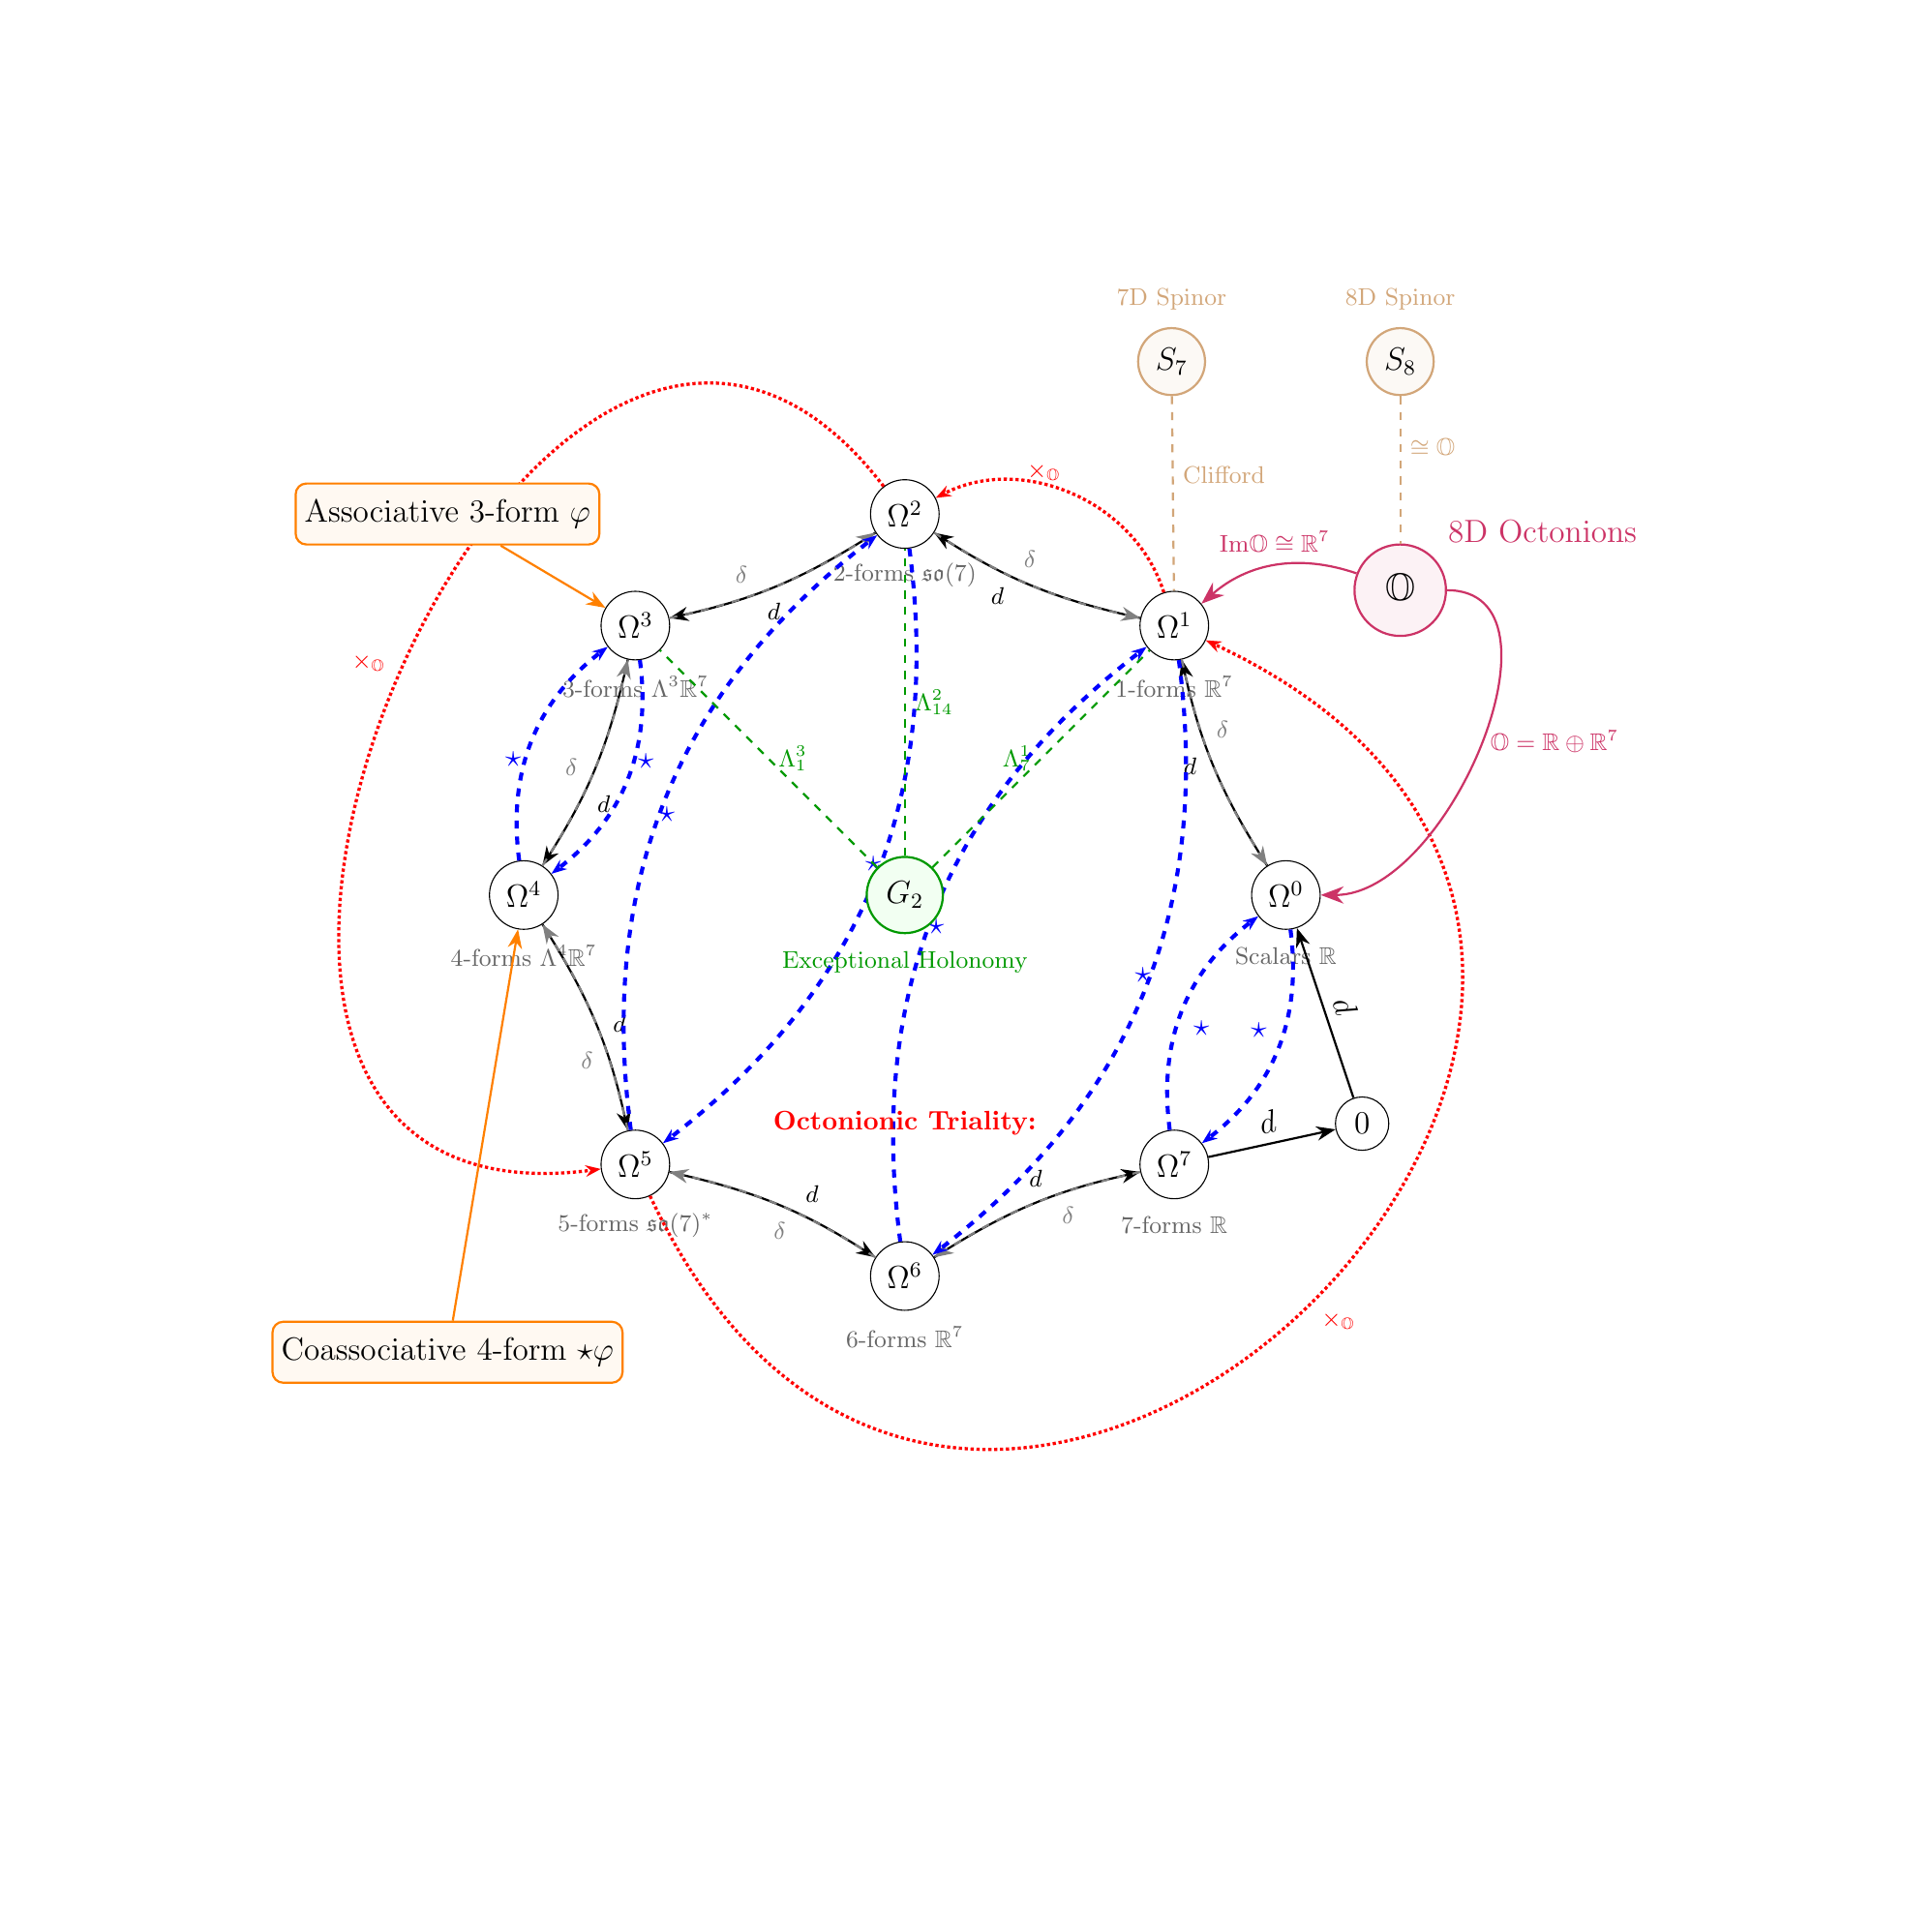
\begin{tikzpicture}[
		node distance=2.5cm and 3cm,
		every node/.style={font=\large},
		arrow/.style={-{Stealth[length=2.5mm]}, thick},
		hodge/.style={blue, dashed, line width=1.5pt, -{Stealth[length=2mm]}},
		triality/.style={red, densely dotted, line width=1.2pt, -{Stealth[length=2mm]}},
		parallel shift/.style={transform canvas={yshift=#1}},
		octonion/.style={draw=purple!80, thick, dashed, rectangle, rounded corners, inner sep=8pt}
		]
		
		% === TITLE ===
		%\node[octonion] at (0, 13) {\Large \textbf{Octonionic Hodge-de Rham Complex: CL(0,7)}};
		
		% === ZERO NODES ===
		%\node[draw, circle, minimum size=0.7cm] (zero0) at (-8, -1) {$0$};
		\node[draw, circle, minimum size=0.7cm] (zero7) at (6, -3) {$0$};
		
		% === OCTONION NODE ===
		\node[draw=purple!80, thick, circle, minimum size=1.2cm, fill=purple!5] 
		(octonions) at (6.5, 4) {\Large $\mathbb{O}$};
		\node[text=purple!80, above right=0.1cm of octonions] {8D Octonions};
		
		% === FORM SPACES IN A CIRCLE ARRANGEMENT ===
		
		% Calculate positions on a circle
		\foreach \i/\deg/\name/\labeltext in {0/0/omega0/{Scalars $\mathbb{R}$},
			1/45/omega1/{1-forms $\mathbb{R}^7$},
			2/90/omega2/{2-forms $\mathfrak{so}(7)$},
			3/135/omega3/{3-forms $\Lambda^3\mathbb{R}^7$},
			4/180/omega4/{4-forms $\Lambda^4\mathbb{R}^7$},
			5/225/omega5/{5-forms $\mathfrak{so}(7)^*$},
			6/270/omega6/{6-forms $\mathbb{R}^7$},
			7/315/omega7/{7-forms $\mathbb{R}$}} {
			\pgfmathsetmacro{\radius}{5}
			\pgfmathsetmacro{\x}{\radius*cos(\deg)}
			\pgfmathsetmacro{\y}{\radius*sin(\deg)}
			\node[draw, circle, minimum size=0.8cm] (\name) at (\x, \y) {$\Omega^{\i}$};
			\node[text=black!60, font=\small] at (\x, \y-0.8) {\labeltext};
		}
		
		% === DE RHAM COMPLEX ARROWS (d) - Outer circle ===
		\foreach \i/\j in {0/1, 1/2, 2/3, 3/4, 4/5, 5/6, 6/7} {
			\draw[arrow] (omega\i) to[bend left=10] node[midway, auto, pos=0.6, font=\small] {$d$} (omega\j);
		}
		
		% 0 → Ω⁰ and Ω⁷ → 0
		\draw[arrow] (zero7) -- node[midway, above, sloped] {$d$} (omega0);
		\draw[arrow] (omega7) -- node[midway, above, sloped] {$d$} (zero7);
		
		% === CODIFFERENTIAL ARROWS (δ) - Inner circle ===
		\foreach \i/\j in {1/0, 2/1, 3/2, 4/3, 5/4, 6/5, 7/6} {
			\draw[arrow, dashed, gray] (omega\i) to[bend right=10] node[midway, auto, pos=0.4, font=\small] {$\delta$} (omega\j);
		}
		
		% === HODGE STAR ARROWS (★) ===
		% CL(0,7): Negative definite metric in 7D: ★² = (-1)^{k(7-k)}
		\draw[hodge] (omega0) to[bend left=30] node[midway, above left] {$\star$} (omega7);
		\draw[hodge] (omega7) to[bend left=30] node[midway, below right] {$\star$} (omega0);
		
		\draw[hodge] (omega1) to[bend left=30] node[midway, above] {$\star$} (omega6);
		\draw[hodge] (omega6) to[bend left=30] node[midway, below] {$\star$} (omega1);
		
		\draw[hodge] (omega2) to[bend left=30] node[midway, above] {$\star$} (omega5);
		\draw[hodge] (omega5) to[bend left=30] node[midway, below] {$\star$} (omega2);
		
		\draw[hodge] (omega3) to[bend left=30] node[midway, above right] {$\star$} (omega4);
		\draw[hodge] (omega4) to[bend left=30] node[midway, below left] {$\star$} (omega3);
		
		% === TRIALITY ARROWS - Special octonionic isomorphisms ===
		\node[text=red, font=\bfseries] at (0, -3) {Octonionic Triality:};
		
		% Ω¹ $\leftrightarrow$ Ω² $\leftrightarrow$ Ω⁵ connections via octonion multiplication
		% The red dashed lines that need cleaing up
		\draw[triality] (omega1) to[bend right=50, looseness=1] 
		node[midway, above left, font=\small] {$\times_{\mathbb{O}}$} (omega2);
		\draw[triality] (omega2) to[bend right=120, looseness=2] 
		node[midway, above left, font=\small] {$\times_{\mathbb{O}}$} (omega5);
		\draw[triality] (omega5) to[bend right=110,, looseness=2.5] 
		node[midway, below right, font=\small] {$\times_{\mathbb{O}}$} (omega1);
		
		% === OCTONION TO FORM SPACES CONNECTIONS ===
		% Octonions decompose as 1 + 7
		\draw[purple!80, thick, -{Stealth[length=3mm]}] 
		(octonions) to[out=0, in=0] node[midway, right, font=\small] {$\mathbb{O} = \mathbb{R} \oplus \mathbb{R}^7$} (omega0);
		\draw[purple!80, thick, -{Stealth[length=3mm]}] 
		(octonions) to[bend right=30] node[midway, above, font=\small] {Im$\mathbb{O} \cong \mathbb{R}^7$} (omega1);
		
		% === G₂ HOLONOMY SPHERE ===
		\node[draw=green!60!black, thick, circle, minimum size=1cm, fill=green!5] 
		(g2) at (0, 0) {$G_2$};
		\node[text=green!60!black, below=0.1cm of g2, font=\small] {Exceptional Holonomy};
		
		% G₂ acts on Ω¹, Ω², Ω³ in special ways
		\draw[green!60!black, thick, dashed] (g2) -- node[midway, left, font=\small] {$\Lambda^1_7$} (omega1);
		\draw[green!60!black, thick, dashed] (g2) -- node[midway, right, font=\small] {$\Lambda^2_{14}$} (omega2);
		\draw[green!60!black, thick, dashed] (g2) -- node[midway, right, font=\small] {$\Lambda^3_1$} (omega3);
		
		% === SPECIAL 3-FORM AND 4-FORM ===
		\node[draw=orange, thick, rectangle, rounded corners, minimum width=2cm, minimum height=0.8cm, fill=orange!5] 
		(associative) at (-6, 5) {Associative 3-form $\varphi$};
		\node[draw=orange, thick, rectangle, rounded corners, minimum width=2cm, minimum height=0.8cm, fill=orange!5] 
		(coassociative) at (-6, -6) {Coassociative 4-form $\star\varphi$};
		
		\draw[orange, thick, -{Stealth[length=2.5mm]}] (associative) -- (omega3);
		\draw[orange, thick, -{Stealth[length=2.5mm]}] (coassociative) -- (omega4);
		
		% === SPINOR CONNECTIONS ===
		\node[draw=brown!70, thick, circle, minimum size=0.8cm, fill=brown!5] 
		(spinor7) at (3.5, 7) {$S_7$};
		\node[draw=brown!70, thick, circle, minimum size=0.8cm, fill=brown!5] 
		(spinor8) at (6.5, 7) {$S_8$};
		\node[text=brown!70, above=0.1cm of spinor7, font=\small] {7D Spinor};
		\node[text=brown!70, above=0.1cm of spinor8, font=\small] {8D Spinor};
		
		% Spinor to form connections
		\draw[brown!70, thick, dashed] (spinor7) -- node[midway, above right, font=\small] {Clifford} (omega1);
		\draw[brown!70, thick, dashed] (spinor8) -- node[midway, above right, font=\small] {$\cong \mathbb{O}$} (octonions);
		
	\end{tikzpicture}
\end{center}

\section{Physical Significance of the Octonionic Hodge-deRham Complex}

The octonionic Hodge-deRham complex for Clifford algebra $\text{CL}(0,7)$ represents one of the most intricate and physically rich structures in modern theoretical physics. Unlike the familiar 3D and 4D cases, this 7-dimensional complex reveals deep connections between exceptional geometry, string theory, and fundamental physics beyond the Standard Model.

\subsection{The Special Status of 7 Dimensions and $G_2$ Holonomy}

The diagram reveals why 7 dimensions hold a privileged position in modern theoretical physics:

\subsubsection{$G_2$ as the Smallest Exceptional Lie Group}
\[
G_2 \subset \text{SO}(7) \quad \text{with} \quad \dim(G_2) = 14
\]
This exceptional Lie group preserves the octonionic structure and decomposes the form spaces in a manner crucial for physics:

\begin{align*}
	\Omega^1(\mathbb{R}^7) &= \Lambda^1_7 \quad &&\text{(Fundamental representation)} \\
	\Omega^2(\mathbb{R}^7) &= \Lambda^2_7 \oplus \Lambda^2_{14} \quad &&\text{where } \Lambda^2_{14} \cong \mathfrak{g}_2 \text{ (adjoint representation)} \\
	\Omega^3(\mathbb{R}^7) &= \Lambda^3_1 \oplus \Lambda^3_7 \oplus \Lambda^3_{27}
\end{align*}

\subsection{Physical Applications in String Theory and M-Theory}

\subsubsection{M-Theory Compactifications}
The central role of $G_2$ holonomy manifolds in M-theory emerges naturally from this complex:

1. M-theory on $G_2$ manifolds: Compactification of 11-dimensional supergravity on 7D $G_2$ holonomy manifolds preserves $\mathcal{N}=1$ supersymmetry in 4D:
\[
\text{M-theory on } \mathbb{R}^{1,3} \times X_{G_2} \to \mathcal{N}=1 \text{ supergravity in 4D}
\]
where $X_{G_2}$ is a $G_2$ manifold.

2. Superpotential from Associative 3-form: The associative 3-form $\varphi \in \Omega^3_1$ generates the superpotential in the effective 4D theory:
\[
W = \int_{X_{G_2}} C \wedge \varphi
\]
where $C$ is the M-theory 3-form field.

3. M2-branes and Calibrated Cycles: Associative 3-cycles (calibrated by $\varphi$) are the natural worldvolumes for M2-branes, while coassociative 4-cycles (calibrated by $\star\varphi$) support magnetic M5-branes.

\subsubsection{String Theory Dualities}
The octonionic triality connecting $\Omega^1$, $\Omega^2$, and $\Omega^5$ manifests in string dualities:

\[
\begin{array}{ccc}
	\Omega^1 & \leftrightarrow & \text{NS-NS sector} \\
	\Omega^2 & \leftrightarrow & \text{R-R sector} \\
	\Omega^5 & \leftrightarrow & \text{D-brane charges}
\end{array}
\]

\subsection{The Associative and Coassociative Forms: Geometric Physics}

\subsubsection{The Associative 3-form $\varphi$}
Defined by octonion multiplication:
\[
\varphi_{ijk} = \langle e_i \times_{\mathbb{O}} e_j, e_k \rangle
\]
This form encodes:
- $G_2$ structure on 7-manifolds
- Calibrations for minimal submanifolds
- Torsion-free condition: $d\varphi = 0$ and $d\star\varphi = 0$ defines a $G_2$ holonomy metric

\subsubsection{The Coassociative 4-form $\star\varphi$}
The Hodge dual satisfies remarkable properties:
\[
\star\varphi = \frac{1}{2}\varphi \wedge \varphi
\]
This relation is crucial for:
- Topological field theory on $G_2$ manifolds
- Donaldson-Thomas invariants in 7 dimensions
- Magnetic dual description in M-theory

\subsection{Octonionic Triality: A Fundamental Symmetry}

The red triality arrows in the diagram represent one of the deepest symmetries in mathematics:

\subsubsection{Mathematical Triality of $\text{Spin}(8)$}
\[
8_v \otimes 8_s \otimes 8_c \quad \text{with symmetry group } S_3
\]
where $8_v$, $8_s$, $8_c$ are vector, spinor, and conjugate spinor representations.

\subsubsection{Physical Manifestations}
1. Superstring theory: Type IIA, IIB, and heterotic dualities
2. U-duality in toroidal compactifications: $E_7(\mathbb{Z}) \supset \text{SL}(2,\mathbb{Z}) \times \text{SO}(6,6;\mathbb{Z})$
3. Three generations in particle physics: Possible connection to the three octonionic division algebras ($\mathbb{R}, \mathbb{C}, \mathbb{H}, \mathbb{O}$)

\subsection{Spinor-Octonion Correspondence}

The relationship $S_8 \cong \mathbb{O}$ between 8-dimensional spinors and octonions is fundamental to:

\subsubsection{Supergravity Theories}
- 11D supergravity: The gravitino $\Psi_M$ is an 8-component spinor in 11 dimensions
- Maximal supersymmetry: $\mathcal{N}=8$ supergravity in 4D has $E_{7(7)}$ symmetry with octonionic structure

\subsubsection{Clifford Algebra $\text{CL}(0,7)$ Representations}
\[
\text{CL}(0,7) \cong \text{Mat}(8,\mathbb{R}) \oplus \text{Mat}(8,\mathbb{R})
\]
The spinor representations:
\[
S_7 = \mathbb{R}^8 \quad \text{(Dirac spinor in 7D)}, \quad S_8 = \mathbb{R}^8 \quad \text{(Majorana spinor)}
\]

\subsection{Hodge Star in 7D: Signature and Physics}

The Hodge star properties in $\text{CL}(0,7)$ (negative definite metric) differ from Lorentzian signatures:

\[
\star^2 = (-1)^{k(7-k)} \quad \text{on } \Omega^k
\]

This leads to:
- Complex structure on middle forms when $\star^2 = -1$
- Real structure when $\star^2 = +1$
- Special implications for self-dual/anti-self-dual equations in 7D gauge theory

\subsection{Flux Compactifications and Moduli Stabilization}

The de Rham complex encodes the moduli space structure of $G_2$ manifolds:

\subsubsection{Moduli Space Metric}
The natural metric on moduli space comes from the Hodge inner product:
\[
\langle \delta\varphi, \delta\varphi \rangle = \int_{X_{G_2}} \delta\varphi \wedge \star\delta\varphi
\]
where $\delta\varphi \in \Omega^3_1$ are infinitesimal deformations of the $G_2$ structure.

\subsubsection{Flux-induced Superpotentials}
Turning on 4-form flux $G \in \Omega^4$ generates a superpotential:
\[
W = \int_{X_{G_2}} G \wedge \varphi
\]
This stabilizes moduli and breaks supersymmetry in a controlled manner.

\subsection{Connections to Particle Physics}

\subsubsection{Exceptional Grand Unification}
The exceptional Lie group $E_6$ contains $G_2$ and provides a natural grand unified theory:
\[
E_6 \supset \text{SO}(10) \times \text{U}(1) \supset \text{SU}(5) \times \text{U}(1)^2
\]
Octonionic structures may explain:
- Three generations of fermions
- Yukawa couplings
- CKM matrix structure

\subsubsection{Higher Gauge Theory}
The forms in the complex correspond to higher gauge fields:
\begin{align*}
	\Omega^1 &: \text{Connection 1-forms} \\
	\Omega^2 &: \text{Curvature 2-forms} \\
	\Omega^3 &: \text{2-gerbe connections (M-theory C-field)} \\
	\Omega^4 &: \text{Field strengths for 3-form gauge fields}
\end{align*}

\subsection{The de Rham Complex as a Quantum Circuit}

Remarkably, the octonionic Hodge-deRham complex resembles quantum computational structures:

\subsubsection{Quantum Information Processing}
- 7 qubit error correction: The $G_2$ code protects against general errors
- Octonionic quantum mechanics: Non-associative generalization of quantum theory
- Topological quantum computing with $G_2$ manifolds

\subsubsection{Holographic Principles}
The 7D bulk theory (described by this complex) relates to 6D boundary theories via holography:
\[
\text{M-theory on } AdS_4 \times X_{G_2} \leftrightarrow \text{CFT}_3 \text{ with } G_2 \text{ symmetry}
\]

\subsection{Conclusion: The Unifying Framework}

The octonionic Hodge-deRham complex for $\text{CL}(0,7)$ provides a unified geometric framework that connects:

1. Exceptional Geometry: $G_2$ holonomy and octonionic structures
2. String/M-theory: Compactifications, dualities, and branes
3. Particle Physics: Grand unification and family structure
4. Quantum Information: Error correction and topological computing
5. Mathematics: Triality, calibrated geometry, and index theory

The diagram is not merely a mathematical curiosity but a roadmap to physics beyond the Standard Model. Each arrow represents a physical transformation or duality, each node a sector of the theory, and the overall structure encodes the symmetries and dynamics of a unified theory of quantum gravity.

The central message is profound: The exceptional structures of octonions and $G_2$ holonomy are not accidental mathematical artifacts but essential ingredients for a complete theory of fundamental physics. The octonionic Hodge-deRham complex shows us precisely how these elements fit together in a coherent, geometrically natural framework.

As research progresses in string theory, exceptional field theory, and quantum gravity, this complex will continue to guide us toward deeper understanding of the universe's mathematical foundations.

	

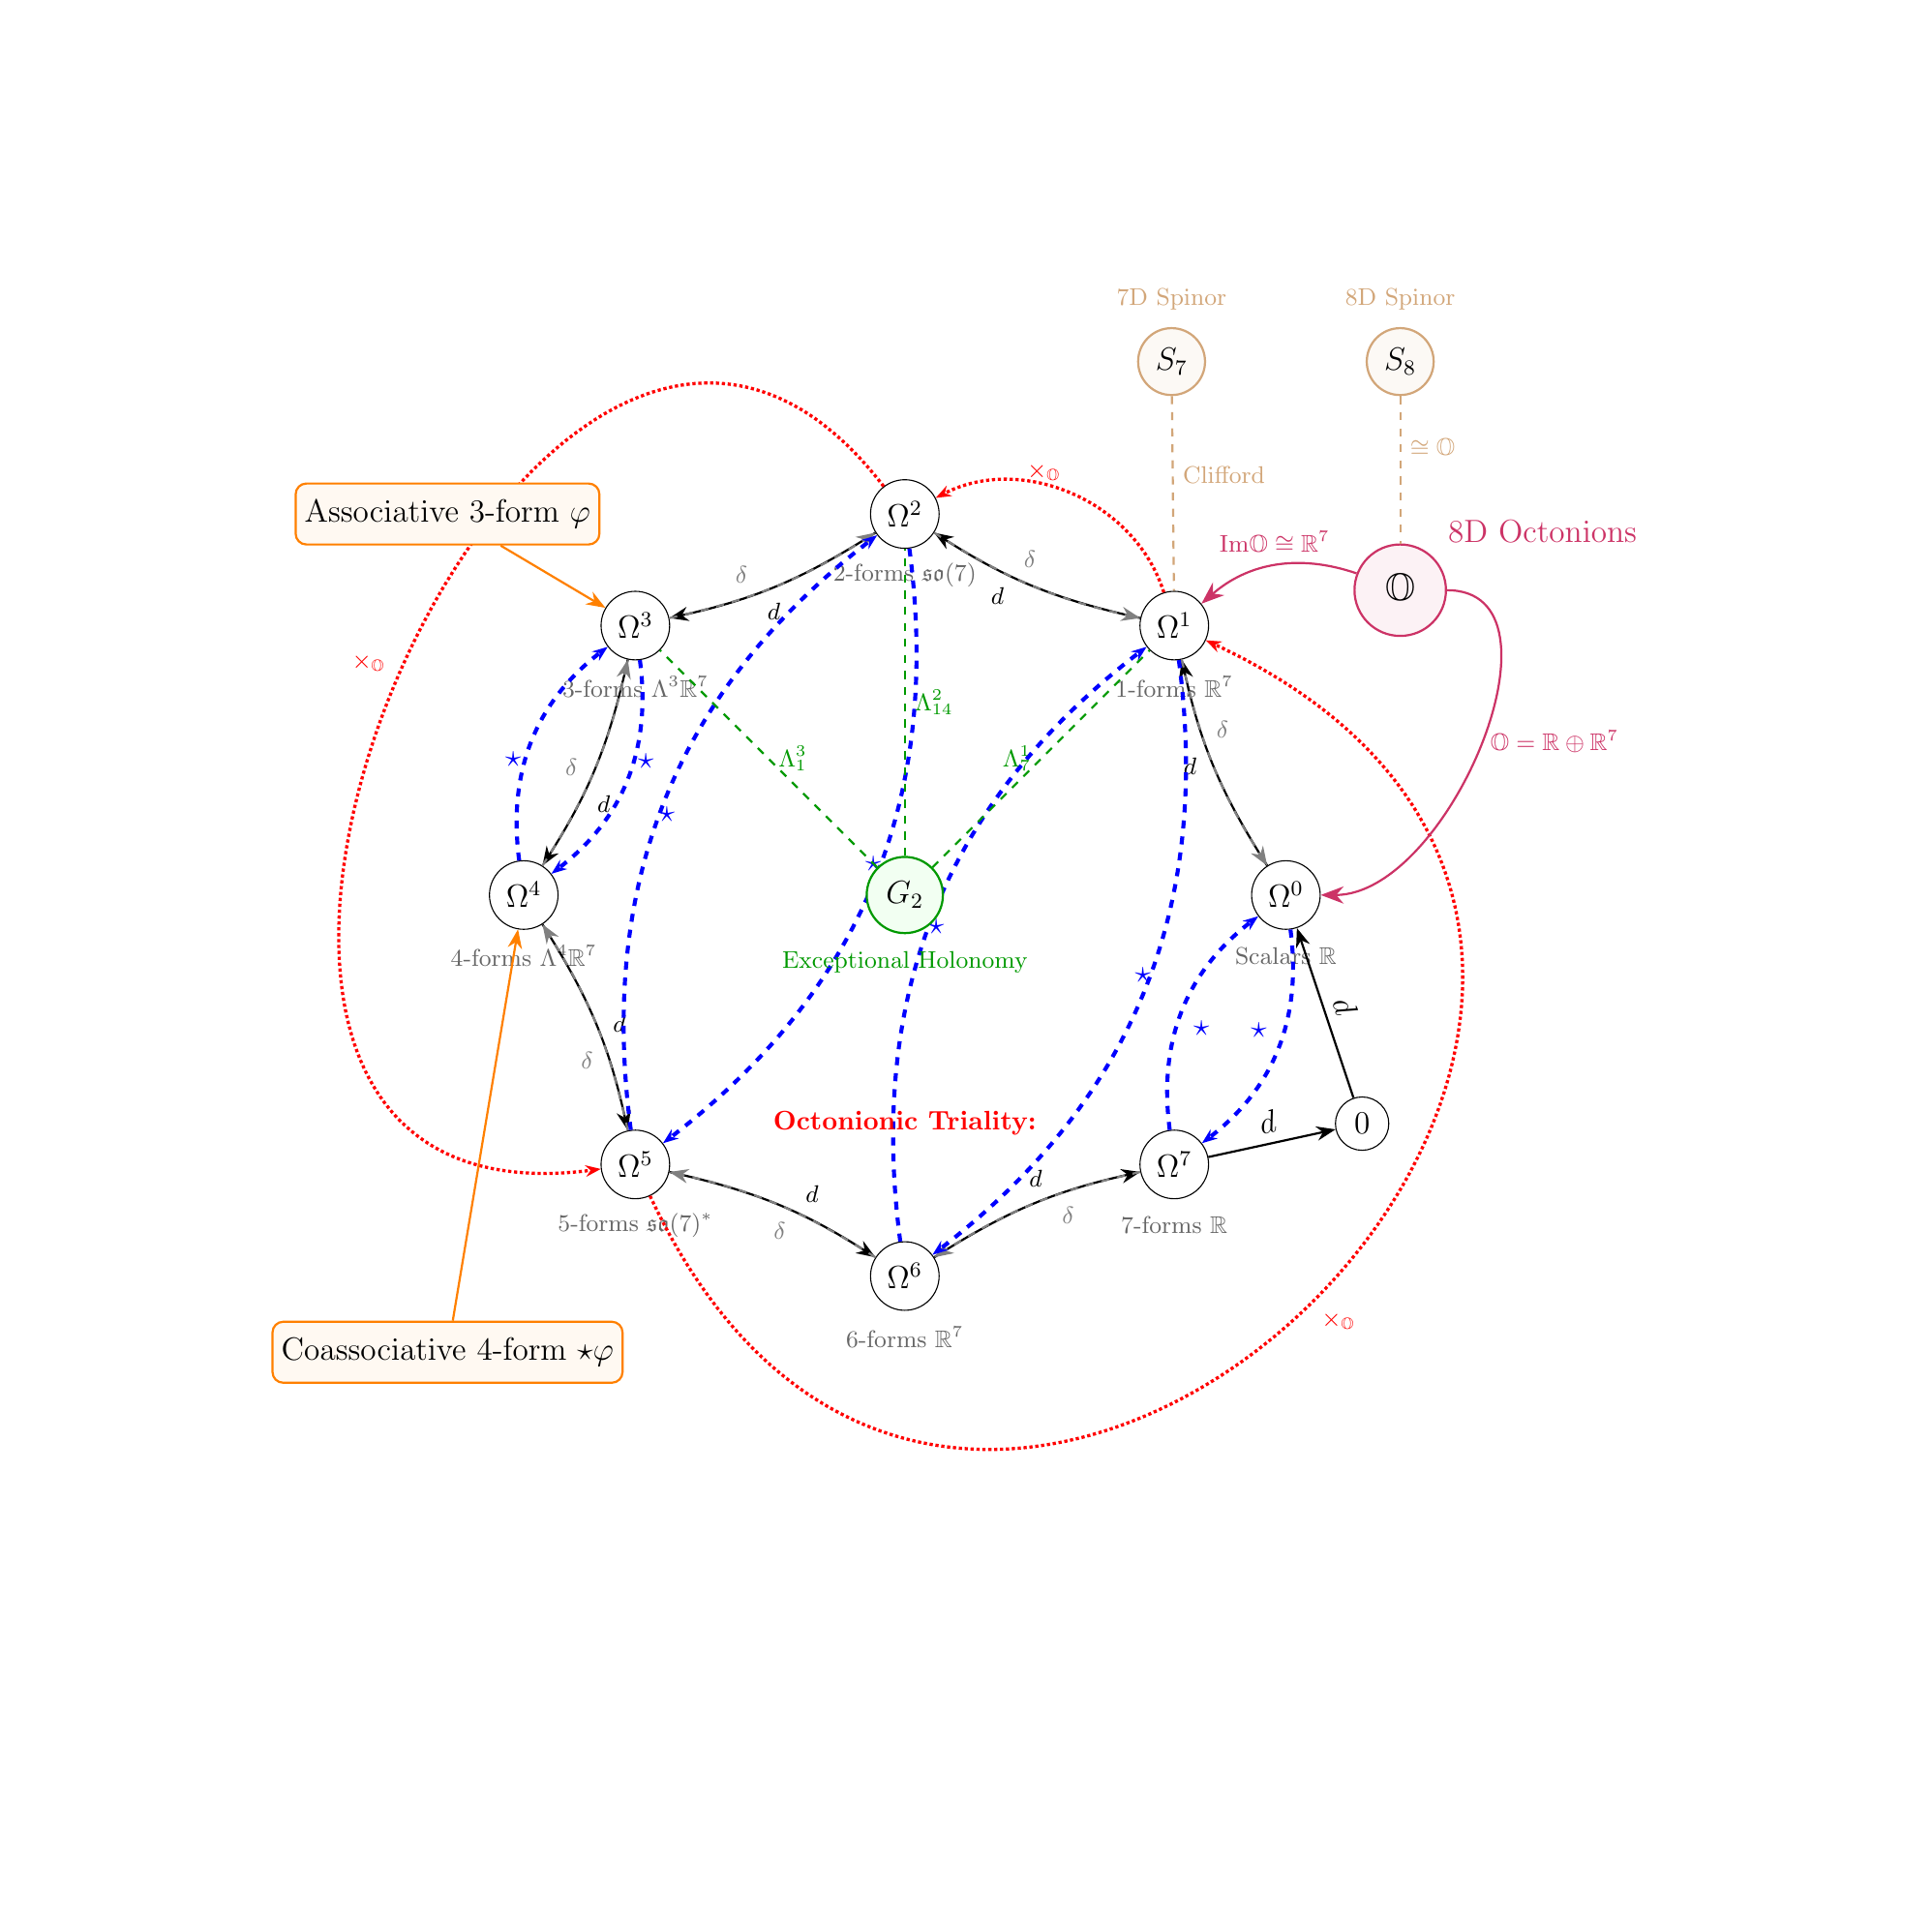
\begin{tikzpicture}[
	node distance=2.5cm and 3cm,
	every node/.style={font=\large},
	arrow/.style={-{Stealth[length=2.5mm]}, thick},
	hodge/.style={blue, dashed, line width=1.5pt, -{Stealth[length=2mm]}},
	triality/.style={red, densely dotted, line width=1.2pt, -{Stealth[length=2mm]}},
	parallel shift/.style={transform canvas={yshift=#1}},
	octonion/.style={draw=purple!80, thick, dashed, rectangle, rounded corners, inner sep=8pt}
	]
	
	% === TITLE ===
	%\node[octonion] at (0, 13) {\Large \textbf{Octonionic Hodge-de Rham Complex: CL(0,7)}};
	
	% === ZERO NODES ===
	%\node[draw, circle, minimum size=0.7cm] (zero0) at (-8, -1) {$0$};
	\node[draw, circle, minimum size=0.7cm] (zero7) at (6, -3) {$0$};
	
	% === OCTONION NODE ===
	\node[draw=purple!80, thick, circle, minimum size=1.2cm, fill=purple!5] 
	(octonions) at (6.5, 4) {\Large $\mathbb{O}$};
	\node[text=purple!80, above right=0.1cm of octonions] {8D Octonions};
	
	% === FORM SPACES IN A CIRCLE ARRANGEMENT ===
	
	% Calculate positions on a circle
	\foreach \i/\deg/\name/\labeltext in {0/0/omega0/{Scalars $\mathbb{R}$},
		1/45/omega1/{1-forms $\mathbb{R}^7$},
		2/90/omega2/{2-forms $\mathfrak{so}(7)$},
		3/135/omega3/{3-forms $\Lambda^3\mathbb{R}^7$},
		4/180/omega4/{4-forms $\Lambda^4\mathbb{R}^7$},
		5/225/omega5/{5-forms $\mathfrak{so}(7)^*$},
		6/270/omega6/{6-forms $\mathbb{R}^7$},
		7/315/omega7/{7-forms $\mathbb{R}$}} {
		\pgfmathsetmacro{\radius}{5}
		\pgfmathsetmacro{\x}{\radius*cos(\deg)}
		\pgfmathsetmacro{\y}{\radius*sin(\deg)}
		\node[draw, circle, minimum size=0.8cm] (\name) at (\x, \y) {$\Omega^{\i}$};
		\node[text=black!60, font=\small] at (\x, \y-0.8) {\labeltext};
	}
	
	% === DE RHAM COMPLEX ARROWS (d) - Outer circle ===
	\foreach \i/\j in {0/1, 1/2, 2/3, 3/4, 4/5, 5/6, 6/7} {
		\draw[arrow] (omega\i) to[bend left=10] node[midway, auto, pos=0.6, font=\small] {$d$} (omega\j);
	}
	
	% 0 → Ω⁰ and Ω⁷ → 0
	\draw[arrow] (zero7) -- node[midway, above, sloped] {$d$} (omega0);
	\draw[arrow] (omega7) -- node[midway, above, sloped] {$d$} (zero7);
	
	% === CODIFFERENTIAL ARROWS (δ) - Inner circle ===
	\foreach \i/\j in {1/0, 2/1, 3/2, 4/3, 5/4, 6/5, 7/6} {
		\draw[arrow, dashed, gray] (omega\i) to[bend right=10] node[midway, auto, pos=0.4, font=\small] {$\delta$} (omega\j);
	}
	
	% === HODGE STAR ARROWS (★) ===
	% CL(0,7): Negative definite metric in 7D: ★² = (-1)^{k(7-k)}
	\draw[hodge] (omega0) to[bend left=30] node[midway, above left] {$\star$} (omega7);
	\draw[hodge] (omega7) to[bend left=30] node[midway, below right] {$\star$} (omega0);
	
	\draw[hodge] (omega1) to[bend left=30] node[midway, above] {$\star$} (omega6);
	\draw[hodge] (omega6) to[bend left=30] node[midway, below] {$\star$} (omega1);
	
	\draw[hodge] (omega2) to[bend left=30] node[midway, above] {$\star$} (omega5);
	\draw[hodge] (omega5) to[bend left=30] node[midway, below] {$\star$} (omega2);
	
	\draw[hodge] (omega3) to[bend left=30] node[midway, above right] {$\star$} (omega4);
	\draw[hodge] (omega4) to[bend left=30] node[midway, below left] {$\star$} (omega3);
	
	% === TRIALITY ARROWS - Special octonionic isomorphisms ===
	\node[text=red, font=\bfseries] at (0, -3) {Octonionic Triality:};
	
	% Ω¹ $\leftrightarrow$ Ω² $\leftrightarrow$ Ω⁵ connections via octonion multiplication
	% The red dashed lines that need cleaing up
	\draw[triality] (omega1) to[bend right=50, looseness=1] 
	node[midway, above left, font=\small] {$\times_{\mathbb{O}}$} (omega2);
	\draw[triality] (omega2) to[bend right=120, looseness=2] 
	node[midway, above left, font=\small] {$\times_{\mathbb{O}}$} (omega5);
	\draw[triality] (omega5) to[bend right=110,, looseness=2.5] 
	node[midway, below right, font=\small] {$\times_{\mathbb{O}}$} (omega1);
	
	% === OCTONION TO FORM SPACES CONNECTIONS ===
	% Octonions decompose as 1 + 7
	\draw[purple!80, thick, -{Stealth[length=3mm]}] 
	(octonions) to[out=0, in=0] node[midway, right, font=\small] {$\mathbb{O} = \mathbb{R} \oplus \mathbb{R}^7$} (omega0);
	\draw[purple!80, thick, -{Stealth[length=3mm]}] 
	(octonions) to[bend right=30] node[midway, above, font=\small] {Im$\mathbb{O} \cong \mathbb{R}^7$} (omega1);
	
	% === G₂ HOLONOMY SPHERE ===
	\node[draw=green!60!black, thick, circle, minimum size=1cm, fill=green!5] 
	(g2) at (0, 0) {$G_2$};
	\node[text=green!60!black, below=0.1cm of g2, font=\small] {Exceptional Holonomy};
	
	% G₂ acts on Ω¹, Ω², Ω³ in special ways
	\draw[green!60!black, thick, dashed] (g2) -- node[midway, left, font=\small] {$\Lambda^1_7$} (omega1);
	\draw[green!60!black, thick, dashed] (g2) -- node[midway, right, font=\small] {$\Lambda^2_{14}$} (omega2);
	\draw[green!60!black, thick, dashed] (g2) -- node[midway, right, font=\small] {$\Lambda^3_1$} (omega3);
	
	% === SPECIAL 3-FORM AND 4-FORM ===
	\node[draw=orange, thick, rectangle, rounded corners, minimum width=2cm, minimum height=0.8cm, fill=orange!5] 
	(associative) at (-6, 5) {Associative 3-form $\varphi$};
	\node[draw=orange, thick, rectangle, rounded corners, minimum width=2cm, minimum height=0.8cm, fill=orange!5] 
	(coassociative) at (-6, -6) {Coassociative 4-form $\star\varphi$};
	
	\draw[orange, thick, -{Stealth[length=2.5mm]}] (associative) -- (omega3);
	\draw[orange, thick, -{Stealth[length=2.5mm]}] (coassociative) -- (omega4);
	
	% === SPINOR CONNECTIONS ===
	\node[draw=brown!70, thick, circle, minimum size=0.8cm, fill=brown!5] 
	(spinor7) at (3.5, 7) {$S_7$};
	\node[draw=brown!70, thick, circle, minimum size=0.8cm, fill=brown!5] 
	(spinor8) at (6.5, 7) {$S_8$};
	\node[text=brown!70, above=0.1cm of spinor7, font=\small] {7D Spinor};
	\node[text=brown!70, above=0.1cm of spinor8, font=\small] {8D Spinor};
	
	% Spinor to form connections
	\draw[brown!70, thick, dashed] (spinor7) -- node[midway, above right, font=\small] {Clifford} (omega1);
	\draw[brown!70, thick, dashed] (spinor8) -- node[midway, above right, font=\small] {$\cong \mathbb{O}$} (octonions);
	
\end{tikzpicture}


\section{Physical Significance of the Octonionic Hodge-deRham Complex}

The octonionic Hodge-deRham complex for Clifford algebra $\text{CL}(0,7)$ represents one of the most intricate and physically rich structures in modern theoretical physics. Unlike the familiar 3D and 4D cases, this 7-dimensional complex reveals deep connections between exceptional geometry, string theory, and fundamental physics beyond the Standard Model.

\subsection{The Special Status of 7 Dimensions and $G_2$ Holonomy}

The diagram reveals why 7 dimensions hold a privileged position in modern theoretical physics:

\subsubsection{$G_2$ as the Smallest Exceptional Lie Group}
\[
G_2 \subset \text{SO}(7) \quad \text{with} \quad \dim(G_2) = 14
\]
This exceptional Lie group preserves the octonionic structure and decomposes the form spaces in a manner crucial for physics:

\begin{align*}
	\Omega^1(\mathbb{R}^7) &= \Lambda^1_7 \quad &&\text{(Fundamental representation)} \\
	\Omega^2(\mathbb{R}^7) &= \Lambda^2_7 \oplus \Lambda^2_{14} \quad &&\text{where } \Lambda^2_{14} \cong \mathfrak{g}_2 \text{ (adjoint representation)} \\
	\Omega^3(\mathbb{R}^7) &= \Lambda^3_1 \oplus \Lambda^3_7 \oplus \Lambda^3_{27}
\end{align*}

\subsection{Physical Applications in String Theory and M-Theory}

\subsubsection{M-Theory Compactifications}
The central role of $G_2$ holonomy manifolds in M-theory emerges naturally from this complex:

1. M-theory on $G_2$ manifolds: Compactification of 11-dimensional supergravity on 7D $G_2$ holonomy manifolds preserves $\mathcal{N}=1$ supersymmetry in 4D:
\[
\text{M-theory on } \mathbb{R}^{1,3} \times X_{G_2} \to \mathcal{N}=1 \text{ supergravity in 4D}
\]
where $X_{G_2}$ is a $G_2$ manifold.

2. Superpotential from Associative 3-form: The associative 3-form $\varphi \in \Omega^3_1$ generates the superpotential in the effective 4D theory:
\[
W = \int_{X_{G_2}} C \wedge \varphi
\]
where $C$ is the M-theory 3-form field.

3. M2-branes and Calibrated Cycles: Associative 3-cycles (calibrated by $\varphi$) are the natural worldvolumes for M2-branes, while coassociative 4-cycles (calibrated by $\star\varphi$) support magnetic M5-branes.

\subsubsection{String Theory Dualities}
The octonionic triality connecting $\Omega^1$, $\Omega^2$, and $\Omega^5$ manifests in string dualities:

\[
\begin{array}{ccc}
	\Omega^1 & \leftrightarrow & \text{NS-NS sector} \\
	\Omega^2 & \leftrightarrow & \text{R-R sector} \\
	\Omega^5 & \leftrightarrow & \text{D-brane charges}
\end{array}
\]

\subsection{The Associative and Coassociative Forms: Geometric Physics}

\subsubsection{The Associative 3-form $\varphi$}
Defined by octonion multiplication:
\[
\varphi_{ijk} = \langle e_i \times_{\mathbb{O}} e_j, e_k \rangle
\]
This form encodes:
- $G_2$ structure on 7-manifolds
- Calibrations for minimal submanifolds
- Torsion-free condition: $d\varphi = 0$ and $d\star\varphi = 0$ defines a $G_2$ holonomy metric

\subsubsection{The Coassociative 4-form $\star\varphi$}
The Hodge dual satisfies remarkable properties:
\[
\star\varphi = \frac{1}{2}\varphi \wedge \varphi
\]
This relation is crucial for:
- Topological field theory on $G_2$ manifolds
- Donaldson-Thomas invariants in 7 dimensions
- Magnetic dual description in M-theory

\subsection{Octonionic Triality: A Fundamental Symmetry}

The red triality arrows in the diagram represent one of the deepest symmetries in mathematics:

\subsubsection{Mathematical Triality of $\text{Spin}(8)$}
\[
8_v \otimes 8_s \otimes 8_c \quad \text{with symmetry group } S_3
\]
where $8_v$, $8_s$, $8_c$ are vector, spinor, and conjugate spinor representations.

\subsubsection{Physical Manifestations}
1. Superstring theory: Type IIA, IIB, and heterotic dualities
2. U-duality in toroidal compactifications: $E_7(\mathbb{Z}) \supset \text{SL}(2,\mathbb{Z}) \times \text{SO}(6,6;\mathbb{Z})$
3. Three generations in particle physics: Possible connection to the three octonionic division algebras ($\mathbb{R}, \mathbb{C}, \mathbb{H}, \mathbb{O}$)

\subsection{Spinor-Octonion Correspondence}

The relationship $S_8 \cong \mathbb{O}$ between 8-dimensional spinors and octonions is fundamental to:

\subsubsection{Supergravity Theories}
- 11D supergravity: The gravitino $\Psi_M$ is an 8-component spinor in 11 dimensions
- Maximal supersymmetry: $\mathcal{N}=8$ supergravity in 4D has $E_{7(7)}$ symmetry with octonionic structure

\subsubsection{Clifford Algebra $\text{CL}(0,7)$ Representations}
\[
\text{CL}(0,7) \cong \text{Mat}(8,\mathbb{R}) \oplus \text{Mat}(8,\mathbb{R})
\]
The spinor representations:
\[
S_7 = \mathbb{R}^8 \quad \text{(Dirac spinor in 7D)}, \quad S_8 = \mathbb{R}^8 \quad \text{(Majorana spinor)}
\]

\subsection{Hodge Star in 7D: Signature and Physics}

The Hodge star properties in $\text{CL}(0,7)$ (negative definite metric) differ from Lorentzian signatures:

\[
\star^2 = (-1)^{k(7-k)} \quad \text{on } \Omega^k
\]

This leads to:
- Complex structure on middle forms when $\star^2 = -1$
- Real structure when $\star^2 = +1$
- Special implications for self-dual/anti-self-dual equations in 7D gauge theory

\subsection{Flux Compactifications and Moduli Stabilization}

The de Rham complex encodes the moduli space structure of $G_2$ manifolds:

\subsubsection{Moduli Space Metric}
The natural metric on moduli space comes from the Hodge inner product:
\[
\langle \delta\varphi, \delta\varphi \rangle = \int_{X_{G_2}} \delta\varphi \wedge \star\delta\varphi
\]
where $\delta\varphi \in \Omega^3_1$ are infinitesimal deformations of the $G_2$ structure.

\subsubsection{Flux-induced Superpotentials}
Turning on 4-form flux $G \in \Omega^4$ generates a superpotential:
\[
W = \int_{X_{G_2}} G \wedge \varphi
\]
This stabilizes moduli and breaks supersymmetry in a controlled manner.

\subsection{Connections to Particle Physics}

\subsubsection{Exceptional Grand Unification}
The exceptional Lie group $E_6$ contains $G_2$ and provides a natural grand unified theory:
\[
E_6 \supset \text{SO}(10) \times \text{U}(1) \supset \text{SU}(5) \times \text{U}(1)^2
\]
Octonionic structures may explain:
- Three generations of fermions
- Yukawa couplings
- CKM matrix structure

\subsubsection{Higher Gauge Theory}
The forms in the complex correspond to higher gauge fields:
\begin{align*}
	\Omega^1 &: \text{Connection 1-forms} \\
	\Omega^2 &: \text{Curvature 2-forms} \\
	\Omega^3 &: \text{2-gerbe connections (M-theory C-field)} \\
	\Omega^4 &: \text{Field strengths for 3-form gauge fields}
\end{align*}

\subsection{The de Rham Complex as a Quantum Circuit}

Remarkably, the octonionic Hodge-deRham complex resembles quantum computational structures:

\subsubsection{Quantum Information Processing}
- 7 qubit error correction: The $G_2$ code protects against general errors
- Octonionic quantum mechanics: Non-associative generalization of quantum theory
- Topological quantum computing with $G_2$ manifolds

\subsubsection{Holographic Principles}
The 7D bulk theory (described by this complex) relates to 6D boundary theories via holography:
\[
\text{M-theory on } AdS_4 \times X_{G_2} \leftrightarrow \text{CFT}_3 \text{ with } G_2 \text{ symmetry}
\]

\subsection{Conclusion: The Unifying Framework}

The octonionic Hodge-deRham complex for $\text{CL}(0,7)$ provides a unified geometric framework that connects:

1. Exceptional Geometry: $G_2$ holonomy and octonionic structures
2. String/M-theory: Compactifications, dualities, and branes
3. Particle Physics: Grand unification and family structure
4. Quantum Information: Error correction and topological computing
5. Mathematics: Triality, calibrated geometry, and index theory

The diagram is not merely a mathematical curiosity but a roadmap to physics beyond the Standard Model. Each arrow represents a physical transformation or duality, each node a sector of the theory, and the overall structure encodes the symmetries and dynamics of a unified theory of quantum gravity.

The central message is profound: The exceptional structures of octonions and $G_2$ holonomy are not accidental mathematical artifacts but essential ingredients for a complete theory of fundamental physics. The octonionic Hodge-deRham complex shows us precisely how these elements fit together in a coherent, geometrically natural framework.

As research progresses in string theory, exceptional field theory, and quantum gravity, this complex will continue to guide us toward deeper understanding of the universe's mathematical foundations.


\section{The Exceptional Jordan Algebra (Albert Algebra)}

The connection between Jordan algebras and the octonionic Hodge-deRham complex reveals one of the deepest structures in exceptional geometry, linking algebraic, geometric, and physical concepts in a remarkably cohesive framework.
At the heart of this connection lies the exceptional Jordan algebra $\mathfrak{J}_3(\mathbb{O})$ - the algebra of $3 \times 3$ Hermitian matrices over the octonions:

\[
\mathfrak{J}_3(\mathbb{O}) = \left\{ 
\begin{pmatrix}
	a & x & \bar{y} \\
	\bar{x} & b & z \\
	y & \bar{z} & c
\end{pmatrix} : a,b,c \in \mathbb{R}, \; x,y,z \in \mathbb{O}
\right\}
\]

This 27-dimensional algebra possesses extraordinary properties:
- Non-associative but power-associative: $(A \circ B) \circ A^2 = A \circ (B \circ A^2)$
- Exceptional: It cannot be realized as a subalgebra of an associative algebra
- Symmetry group: Its automorphism group is the exceptional Lie group $F_4$

\subsection{Jordan Algebra $\leftrightarrow$ Form Decomposition Correspondence}

The decomposition of differential forms under $G_2$ directly corresponds to the structure of $\mathfrak{J}_3(\mathbb{O})$:

\begin{center}
	\begin{tabular}{c|c|c}
		\textbf{Form Space} & \textbf{G$_2$ Decomposition} & \textbf{Jordan Algebra Component} \\
		\hline
		$\Omega^0$ & $\mathbb{R}$ & Trace part: $\text{tr}(J)$ \\
		$\Omega^1$ & $\Lambda^1_7$ & Off-diagonal octonions: $x,y,z \in \text{Im}\mathbb{O}$ \\
		$\Omega^2$ & $\Lambda^2_7 \oplus \Lambda^2_{14}$ & $\Lambda^2_7$ corresponds to Jordan multiplication \\
		$\Omega^3$ & $\Lambda^3_1 \oplus \Lambda^3_7 \oplus \Lambda^3_{27}$ & $\Lambda^3_{27} \cong \mathfrak{J}_3(\mathbb{O})_0$ (traceless part) \\
		$\Omega^4$ & $\Lambda^4_1 \oplus \Lambda^4_7 \oplus \Lambda^4_{27}$ & Hodge dual of $\Omega^3$ decomposition
	\end{tabular}
\end{center}

The key isomorphism is:
\[
\Lambda^3_{27} \cong \mathfrak{J}_3(\mathbb{O})_0 \quad \text{(27-dimensional traceless Jordan matrices)}
\]

\subsection{The Freudenthal Triple System}

The connection extends to the Freudenthal triple system $\mathfrak{F}(\mathbb{O})$, which combines the Jordan algebra with its dual:

\[
\mathfrak{F}(\mathbb{O}) = \mathbb{R} \oplus \mathbb{R} \oplus \mathfrak{J}_3(\mathbb{O}) \oplus \mathfrak{J}_3(\mathbb{O})
\]

This 56-dimensional system has symmetry group $E_7$, and its geometry is encoded in the Hodge star relations in the octonionic complex.

\subsubsection{Magic Square Construction}
The exceptional Lie groups form the "magic square" via Jordan algebras:

\[
\begin{array}{c|cccc}
	& \mathbb{R} & \mathbb{C} & \mathbb{H} & \mathbb{O} \\
	\hline
	\mathbb{R} & \text{SO}(3) & \text{SU}(3) & \text{Sp}(3) & F_4 \\
	\mathbb{C} & \text{SU}(3) & \text{SU}(3)^2 & \text{SU}(6) & E_6 \\
	\mathbb{H} & \text{Sp}(3) & \text{SU}(6) & \text{SO}(12) & E_7 \\
	\mathbb{O} & F_4 & E_6 & E_7 & E_8
\end{array}
\]

\subsection{Physical Manifestations of the Jordan Structure}

\subsubsection M-Theory and Black Hole Entropy
The 27-dimensional $\mathfrak{J}_3(\mathbb{O})$ appears in M-theory compactifications:

- Black hole charges in 5D are described by Jordan algebra elements
- Entropy formula: $S = \pi \sqrt{\det(J)}$ where $J \in \mathfrak{J}_3(\mathbb{O})$
- U-duality: The $E_6$ symmetry acts on the 27 charges

\subsubsection{Exceptional Field Theory (ExFT)}
In ExFT, the internal metric becomes an element of the exceptional Jordan algebra:

\[
\mathcal{M}_{MN} \in E_6/\text{USp}(8) \quad \text{parameterized by } \mathfrak{J}_3(\mathbb{O})
\]

The section condition in ExFT has a natural interpretation in terms of Jordan algebraic constraints.

\subsubsection{String Theory Moduli Spaces}
The moduli space of type IIB string theory on $T^2$ is:
\[
\text{SL}(2,\mathbb{R})/\text{SO}(2) \times \text{SO}(6,6)/(\text{SO}(6)\times\text{SO}(6))
\]
which embeds into $E_7/\text{SU}(8)$, with Jordan structure controlling quantum corrections.

\subsection{Jordan Algebraic Operations in the Hodge-deRham Complex}

The Jordan product $\circ$ appears geometrically in several ways:

\subsubsection 1. Metric from Jordan Trace Form
The inner product on forms can be expressed via Jordan trace:
\[
\langle \omega, \eta \rangle = \text{Tr}(J_\omega \circ J_\eta)
\]
where $J_\omega, J_\eta \in \mathfrak{J}_3(\mathbb{O})$ correspond to forms.

\subsubsection{Associative 3-form as Jordan Determinant}
The associative 3-form $\varphi$ corresponds to the Jordan determinant:
\[
\det(J) = \frac{1}{3}\text{Tr}(J^3) - \frac{1}{2}\text{Tr}(J^2)\text{Tr}(J) + \frac{1}{6}\text{Tr}(J)^3
\]
For the identity element $J = I$, $\det(I) = 1$ gives the normalized volume form.

\subsubsection 3. Jordan Triple Product and Curvature
The Riemann curvature tensor can be expressed using the Jordan triple product:
\[
\{X,Y,Z\} = (X \circ Y) \circ Z + (Z \circ Y) \circ X - (X \circ Z) \circ Y
\]

\subsection{The 27 $\rightarrow$ 7 + 14 + 6 Decomposition}

Under $G_2 \subset \text{SO}(7)$, the 27-dimensional representation decomposes as:
\[
\mathbf{27} \rightarrow \mathbf{1} \oplus \mathbf{7} \oplus \mathbf{14} \oplus \mathbf{5}
\]
But wait - $G_2$ has no 5-dimensional irreducible representation! Actually, the correct decomposition is more subtle due to the non-associativity of octonions.

The proper decomposition under $G_2$ is:
\[
\mathfrak{J}_3(\mathbb{O}) = \mathbb{R} \oplus V_7 \oplus V_{14} \oplus \mathcal{R}
\]
where $\mathcal{R}$ is a 6-dimensional reducible representation that further decomposes under additional symmetry.

\subsection{Connection to the Hodge Star Operation}

The Hodge star $\star: \Omega^k \to \Omega^{7-k}$ induces a Jordan algebraic duality:

\subsubsection{$\Omega^3_{27} \leftrightarrow \Omega^4_{27}$ Duality}
The Hodge star restricts to an isomorphism between the 27-dimensional components:
\[
\star: \Lambda^3_{27} \xrightarrow{\cong} \Lambda^4_{27}
\]
This corresponds to the Freudenthal duality in the Jordan algebra:
\[
J \mapsto \tilde{J} = \star J \quad \text{with} \quad \tilde{\tilde{J}} = (-1)J
\]

\subsection{Physics of Jordan Algebraic Structures}

\subsubsection{M2-brane Moduli Space}
The moduli space of $N$ coincident M2-branes is conjectured to be related to $\mathfrak{J}_3(\mathbb{O})^N$ modulo some symmetry.

\subsubsection{Exceptional Chern-Simons Theory}
A 3D Chern-Simons theory with gauge group $F_4$ or $E_6$ naturally involves the Jordan algebra in its Lagrangian:
\[
\mathcal{L} \sim \epsilon^{\mu\nu\rho} \text{Tr}\left(A_\mu \partial_\nu A_\rho + \frac{2}{3}A_\mu A_\nu A_\rho\right) + \text{Tr}(J \circ D_\mu J)
\]

\subsubsection{Conformal Field Theories}
The 6D $(2,0)$ superconformal theory has moduli space described by $\mathfrak{J}_3(\mathbb{O})$, explaining its exceptional symmetry.

\subsection{The Octonionic Hodge-deRham as Jordan Algebraic Calculus}

The entire complex can be reinterpreted through Jordan algebra glasses:

\begin{center}
	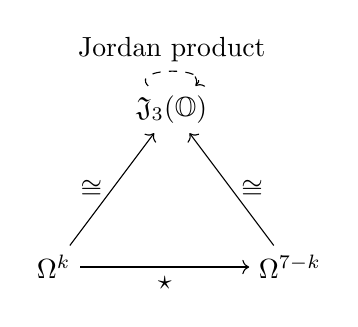
\begin{tikzpicture}[node distance=2cm]
		\node (d) at (0,0) {$\Omega^k$};
		\node (star) at (3,0) {$\Omega^{7-k}$};
		\node (J) at (1.5,2) {$\mathfrak{J}_3(\mathbb{O})$};
		
		\draw[->] (d) -- node[below] {$\star$} (star);
		\draw[->] (d) -- node[left] {$\cong$} (J);
		\draw[->] (star) -- node[right] {$\cong$} (J);
		\draw[->, dashed] (J) to[out=135, in=45, looseness=1.5] node[above] {Jordan product} (J);
	\end{tikzpicture}
\end{center}

\subsubsection{Differential Operators as Jordan Derivations}
The exterior derivative $d$ corresponds to Jordan derivations:
\[
D_X(Y) = X \circ Y - Y \circ X \quad \text{for} \quad X,Y \in \mathfrak{J}_3(\mathbb{O})
\]

The condition $d^2 = 0$ translates to:
\[
D_X D_Y + D_Y D_X = D_{X \circ Y}
\]
which is the defining relation for Jordan operator algebras.

\subsection{Quantum Mechanics and Jordan Algebras}

Pascual Jordan's original motivation was to develop an algebraic formulation of quantum mechanics. The exceptional Jordan algebra represents a non-associative generalization of quantum observables:

\subsubsection{Quantum Observables}
In standard QM: Observables = Hermitian matrices (associative)
In exceptional QM: Observables = $\mathfrak{J}_3(\mathbb{O})$ (non-associative)

The probability postulate becomes:
\[
P(\psi) = \frac{\langle \psi | J | \psi \rangle}{\text{Tr}(J)}
\]
where $|\psi\rangle$ is an octonionic state vector.

\subsection{String Theory Landscape and Jordan Structure}

The landscape of string vacua has an algebraic structure related to Jordan algebras:

\subsubsection{Vacuum Moduli Space}
The moduli space of M-theory on $G_2$ manifolds is:
\[
\mathcal{M} = \frac{E_6(\mathbb{Z}) \backslash E_6(\mathbb{R})}{\text{USp}(8)}
\]
which is parameterized by Jordan algebra elements modulo discrete symmetries.

\subsubsection{Yukawa Couplings as Jordan Products}
Yukawa couplings in string compactifications can be computed as:
\[
Y_{ijk} = \int_X \Omega_i \wedge \Omega_j \wedge \Omega_k
\]
which corresponds to the Jordan triple product $\{J_i, J_j, J_k\}$.

\subsubsection{Flux Quantization}
Flux quantization conditions become Jordan algebraic constraints:
\[
[G_4] \in H^4(X, \mathbb{Z}) \quad \leftrightarrow \quad \text{det}(J) \in \mathbb{Z}
\]

\subsection{Conclusion: The Jordan-Algebraic Nature of Exceptional Geometry}

The octonionic Hodge-deRham complex is not merely a differential complex but a Jordan-algebraic calculus where:

1. Forms $\leftrightarrow$ Jordan algebra elements
2. Hodge star $\leftrightarrow$ Freudenthal duality
3. Exterior derivative $\leftrightarrow$ Jordan derivation
4. Associative 3-form $\leftrightarrow$ Jordan determinant
5. $G_2$ action $\leftrightarrow$ Jordan automorphisms

This perspective reveals why exceptional structures ($G_2$, $F_4$, $E_6$, $E_7$, $E_8$) appear so prominently in modern theoretical physics: they are the symmetry groups of the fundamental algebraic structures (division algebras and Jordan algebras) that underpin quantum gravity.

The diagram connecting octonions, differential forms, spinors, and $G_2$ holonomy is thus unified by the exceptional Jordan algebra $\mathfrak{J}_3(\mathbb{O})$, which serves as the coordinate ring for exceptional geometry. Every arrow in the octonionic Hodge-deRham complex can be interpreted as a Jordan-algebraic operation, revealing a deep coherence between algebra, geometry, and physics that points toward a truly unified theory.

\end{document}




